%& -shell-escape_
\documentclass[12pt]{article}
\usepackage{infocourse}
%opening
\title{,,Теория информации``.\\ Лекции 1-8}
\author{А.В. Смаль}

\begin{document}

\maketitle
            
\section{Комбинаторный подход}
\subsection{Информация по Хартли}
Пусть задано некоторое конечное множество \(A\)~--- \emph{множество исходов}.
\begin{definition}[1928]
Определим \emph{количество информации в \(A\)} как \(\chi(A) = \log_2|A|\) (мы будем измерять количество информации в битах, поэтому все логарифмы будут по основанию \(2\), для байтов основание нужно было бы заменить на \(256\)).
\end{definition}

Если про некоторый \(x\in A\) стало известно, что \(x\in B\), то теперь для идентификации \(x\) нам достаточно \(\chi(A\cap B) = \log |A\cap B|\) битов, т.е. нам сообщили \(\chi(A) - \chi(A\cap B)\) битов информации.

\begin{example}
    Предположим, что мы хотим узнать некоторое неизвестное упорядочение множества $\{\seqn{a}{5}\}$. Нам стало известно,
    что \(a_1>a_2\) или \(a_3>a_4\). Сколько битов информации мы узнали? Множество \(A\) состоит из \(5!\) перестановок,
    множество \(B\)~--- из перестановок, которые удовлетворяют новому условию. Легко проверить, что \(|B| = 90\). Итого
    мы узнали \(\log 120 - \log 90 = \log(4/3)\) битов.
\end{example}

Пусть \(A\subset\bitstr\times\bitstr\). Обозначим через \(\pi_1(A)\) и \(\pi_2(A)\) проекции множества \(A\) на первую и вторую координату соответственно, а \(\chi_1(A) = \log|\pi_1(A)|\) и \(\chi_2(A) = \log|\pi_2(A)|\)~--- их сложность по Хартли.

\begin{theorem} 
\(\chi(A) \le \chi_1(A) + \chi_2(A)\).
\end{theorem}

\begin{definition}
Количество информации в второй компоненте \(A\) при известной первой
\[\chi_{2|1} = \log\left(\max_{a\in\pi_1(A)} |A_a|\right),\]
где $A_a = \{(a, x) \mid x\in \pi_2(A)\}$.
\end{definition}

\begin{theorem} 
\(\chi(A) \le \chi_1(A) + \chi_{2|1}(A)\).
\end{theorem}

\begin{theorem}\label{thm:volume}
Для \(A\subset\bitstr\times\bitstr\times\bitstr\)
\[2\cdot\chi(A) \le \chi_{12}(A) + \chi_{13}(A) + \chi_{23}(A).\]
\end{theorem}
\begin{corollary}
Квадрат объёма трёхмерного тела не превосходит произведение площадей его проекций на координатные плоскости.
\end{corollary}

\begin{statement}
Если \(f: X\to Y\)
\begin{enumerate}
    \item является сюръекцией, то \(\chi(Y)\le \chi(X)\),
    \item является инъекцией, то \(\chi(X)\le \chi(Y)\).
\end{enumerate}
\end{statement}

\subsection{Применение: игра в 10 вопросов}
Сколько вопросов на ДА/НЕТ нужно задать, чтобы определить загаданное число от 1 до \(N\), если (a) можно задавать вопросы адаптивно; (б) вопросы нужно написать на бумажке заранее.

Оценка \(\lceil\log N\rceil \) достигается в обоих случаях, если задавать вопросы про биты двоичного представления загаданного числа.

Докажем нижнюю оценку. Пусть \(A=[N]\). Множество \(Q = \{(\seqn{q}{k})\}\)~--- множество протоколов (ответы на вопросы). 
Можно рассматривать \(A\) и \(Q\) как проекции некоторого множества исходов игры \(S\) на разные координаты. Тогда верны следующие неравенства:
\begin{itemize}
\item \( \chi_Q(S) = \chi(Q) \le \chi_1(Q) + \chi_2(Q) + \dotsb + \chi_k(Q) \le k, \)
\item \( \chi_A(S) = \chi(A) \le \chi(S) \le \chi_Q(S) + \chi_{A|Q}(S) \le k + 0 = k. \)
\end{itemize}
Таким образом получаем, что \(\log N = \chi(A) \le k\).

\subsection{Цена информации}
Пусть имеется некоторое неизвестное число от 1 до \(n\) (где \(n\ge2)\).
Разрешается задавать любые вопросы с ответами ДА/НЕТ. При ответе ДА мы
заплатим 1 рубль, а при ответе НЕТ~— два рубля. Сколько необходимо и достаточно заплатить для отгадывания числа?

\paragraph{Верхняя оценка.} Давайте задавать вопросы так, чтобы отрицательные ответы приносили в два раза больше информации, чем положительные. Тогда за каждый бит информации мы заплатим \(c\log n\) для некоторой константы \(c\). Пусть вопросы будут вида ,,\(x\in T\)?``. Тогда требуется
\[2(\log |X| - \log|X \cap T|) = \log |X| - \log|X\cap\overline T|.\]
Пусть \(|X \cap T| = \alpha|X|\), тогда \(|X\cap\overline T| = (1 - \alpha)|X|\),
т.о. \(\alpha^2 = 1 - \alpha\), \(\alpha=(\sqrt 5 - 1) / 2\). При любом ответе мы заплатим \(c = 1/(-\log \alpha)\approx 1.44\) рублей за бит, а в целом~— \(\log n / (-\log\alpha)\) рублей.

\paragraph{Нижняя оценка.} Применим рассуждение про злонамеренного противника (adversary argument). Пусть противник
выбирает ответ ДА/НЕТ в зависимости от того, какое из двух значение \(1/(\log |X| - \log|X \cap T|)\) и \((2/\log |X| -
\log|X \cap \overline T|)\) больше. При любых \(X,\ T\) одно из этих значений не меньше \(c = 1/(-\log\alpha)\). Таким
образом мы заставляем алгоритм платить не менее \(c\) рублей за бит, а значит любой алгоритм в худшем случае заплатит
\(\lceil c\log n\rceil\) рублей.

\subsection{Применение: упорядочивание камней по весу}
\subsubsection{Верхняя и нижняя оценки для произвольного $N$}
Сколько сравнений нужно сделать для того, чтобы упорядочить \(N\) камней по весу?

\paragraph{Нижняя оценка.} Потребуется \(\lceil\chi(S_N)\rceil = \lceil\log n!\rceil\) сравнений.  

\paragraph{Верхняя оценка.} Будем сортировать вставкой с бинарным поиском места вставки. Количество сравнений:
\[
\lceil\log 2\rceil + \lceil\log 3\rceil +\dotsb+ \lceil\log n\rceil \le \log n! + n - 1 = n\log n + O(n).
\]

\subsubsection{Точные оценки для маленьких $N$}
\begin{exercise}
Сколько нужно взвешиваний, чтобы упорядочить \(N\) камней по весу? 
Найдите точный ответ на этот вопрос для \(N = 2, 3, 4, 5\). Указание: воспользуйтесь жадной стратегией, при которой каждое взвешивание приносит максимум информации.
\end{exercise}

\subsection{Применение: поиск фальшивой монетки}
\begin{itemize}
\item 20 монет, одна фальшивая легче остальных.

Каждое взвешивание даёт не более \(\log 3\) битов. 
Итого \(k\ge\log N/\log 3 = \log_3 N\).

\item 13 монет, одна фальшивая (с неизвестным относительным весом), 3 взвешивания.

Два варианта первого шага:
\begin{itemize}
\item если взвешиваем по 4, то при равенстве нельзя из 5 за два взвешивания найти фальшивую (остаётся 10 исходов),
\item если взвешиваем по 5, то при неравенстве остаётся 10 возможных исходов.
\end{itemize}

\item 15 монет, одна фальшивая, три взвешивания. Не требуется узнавать относительный вес монеты.

Всего исходов \(2\cdot 14 + 1 > 27\), т.к. только в случае трёх равенств мы можем не узнать относительный вес фальшивой монеты.

\item 14 монет, одна фальшивая, три взвешивания. Не требуется узнавать относительный вес монеты.

Всего исходов \(2\cdot 13 + 1 \le 27\), но определить тем не менее нельзя. Аппарата информации по Хартли недостаточно.

\end{itemize}

\subsection{Логика знаний}
В этом разделе мы будем называть множество исходов $A$ множеством \emph{миров}.
Пусть $f$~--- это некоторая функция из $A$ в некоторое множество $I$ (будем воспринимать это как информация о мире).
Нам не важно какие значения принимает $f$, нам будут важны лишь классы эквивалентности, на которые $f$ разбивает $A$:
каждый класс эквивалентности будет состоять из миров $A$ с одинаковым значением $f$.

\begin{example}
    Пусть $A = \{1,2,3,4,5\}$, а $f(x) = x \bmod 3$. Тогда $f$ разбивает $A$ на три класса эквивалентности 
    $\{1,4\}$, $\{2,5\}$ и $\{3\}$.
\end{example}

Пусть $B\subset A$~--- это некоторое \emph{утверждение} о мирах. $B$ \emph{истинно} в мире $x$, если $x\in B$.
В противном случае $B$ \emph{ложно} в $x$. В мире $x$ мы \emph{знаем, что $B$ истинно}, если $y \in B$ для всех 
$y\sim x$.

\begin{example}
    Пусть $A = \{1,2,3,4,5\}$, а $f(x) = x \bmod 3$. Тогда в мирах $1$, $4$ и $3$ мы знаем, 
    что мир меньше $5$.  А в мирах $2$ и $5$~--- не знаем.
\end{example}
\begin{remark}
    ,,Не знаем`` мы будем понимать в смысле ,,не верно, что знаем``.
\end{remark}

К утверждениям о мирах можно применять обычные логические связки: <<И>> (пересечение), <<ИЛИ>> (объединение),
<<НЕ>> (дополнение).

\begin{statement}
    Если в мире $x$ мы знаем $B$, то в мире $x$ мы знаем, что мы знаем $B$.
    Аналогично, если в мире $x$ мы не знаем $B$, то в мире $x$ мы знаем, что не знаем $B$.
\end{statement}

Пусть теперь у нас есть $k$ человек со своими знаниями о мире. 
Они определяют $k$ отношений эквивалентности $\sim_1,\sim_2,\dotsc,\sim_k$ и,
соответственно, $k$ разбиений на классы эквивалентности.

\begin{example}
    Пусть множество миров $A = \{1,2,3,4,5\}$ и есть два человека, Алиса и Боб.
    Алиса знает значения $f_A(x) = x \bmod 3$, а Боб знает $f_B(x) = x\bmod 2$.
    Тогда классы эквивалентности Алисы: $\{1,4\}$, $\{2,5\}$ и $\{3\}$,
    а классы эквивалентности Боба:  $\{1,3,5\}$ и $\{2,4\}$.
    В мире 1 Алиса знает, что мир меньше 5, а Боб не знает. В мире 4 они оба это знают.
    В мире 1 Алиса не знает, что Боря не знает, что мир меньше 5 (действительно, в мире 4,
    который с точки зрения Алисы эквивалентен 1, Боря это знает).
\end{example}

\section{Вероятностный подход}
\subsection{Энтропия Ш\'{е}ннона}

Энтропия Шеннона определяет количество информации \(H(\alpha)\) в распределении
вероятностей для некоторой случайной величины \(\alpha\).  Пусть \(\alpha\)
принимает значения из множества \(\{\seqn{a}{k}\}\) с вероятностями
\(\{\seqn{p}{k}\}\), \(p_i\ge 0 \), \(\sum_ip_i=1\).

Нам бы хотелось, чтобы это определение согласовывалось с определением Хартли, т.е. имеют место следующие ,,граничные условия``:
\begin{itemize}
\item если \(p_1=\dotsb=p_k\), то \(H(\alpha) = \log k\),
\item если \(p_1=1\), \(p_2=\dotsb=p_k=0\), то \(H(\alpha) = 0\).
\end{itemize}
Будем искать \(H(\alpha)\) в виде математического ожидания ,,удивления`` от исхода случайной величины (,,удивление`` зависит от вероятности данного исхода).
\[H(\alpha) = \sum_i p_i\cdot \mathrm{impress}(p_i).\]
Граничные условия однозначно определяют функцию \(\mathrm{impress}(p_i) = \log\frac{1}{p_i} = -\log p_i\).
\begin{definition}[1948]
Энтропия Шеннона случайной величины \(\alpha\) 
\[
H(\alpha) = \sum_{i=1}^k p_i\cdot\log\frac1p_i.
\]
(По непрерывности доопределим \(0\cdot \log\frac10 = 0\).)
\end{definition}

Можно вывести это соотношение из определения Хартли более формально. 
Пусть $W_n$~--- это множество всех слов длины $n$ состоящих из букв $\{\seqn{a}{k}\}$,
где каждая буква $a_i$ встречается ровно $n_i = p_i\cdot n$ раз
(будем считать, что вероятности $p_i$ рациональны, и что множество 
$W_n$ определено только тогда, когда все $n_i$ целые).
Информация по Хартли в $W_n$ 
\[
    \chi(W_n) = \log |W_n| = \log \frac{n!}{n_1!n_2!\dotsb n_k!}.
\]
Это выражение можно оценить при помощи формулы Стирлинга.
\[
    \begin{aligned}
    \chi(W_n)&\ =  \log \frac{\poly(n)\cdot (n/e)^n}
    {\poly(n)\cdot(n_1/e)^{n_1}\cdot(n_1/e)^{n_2}\dotsm(n_k/e)^{n_k}} =\\
    &\ = \log \left(\left(\frac{n}{n_1}\right)^{n_1}\cdot
                    \left(\frac{n}{n_2}\right)^{n_2}\dotsm
                    \left(\frac{n}{n_k}\right)^{n_k}\right) + O(\log n) =\\
    &\ = \log \left(\left(\frac{1}{p_1}\right)^{p_1\cdot n}\cdot
                    \left(\frac{1}{p_2}\right)^{p_2\cdot n}\dotsm
                    \left(\frac{1}{p_k}\right)^{p_k\cdot n}\right) + O(\log n) =\\
    &\ = n \cdot \sum_{i=1}^k p_i \cdot \log\frac{1}{p_i} + O(\log n).
    \end{aligned}
\]
В среднем на один символ приходится $\chi(W_n)/n$ битов информации.
В пределе получаем
\[
    \lim_{n\to \infty}\frac{\chi(W_n)}{n} = \sum_{i=1}^k p_i \cdot \log\frac{1}{p_i} = H(\alpha)
\]
(предел нужно брать по бесконечной подпоследовательности натуральных чисел $n$ таких,
для которых все $\{n_i\}$~--- целые).
 

\begin{lemma}\label{lm:entropy-properties}
Для энтропии Шеннона выполняются следующие соотношения.
\begin{itemize}
\item \(H(\alpha) \ge 0\), причём \(H(\alpha) = 0\) \(\iff\) распределение \(\alpha\) вырождено.

\item \(H(\alpha) \le \log k\), причём \(H(\alpha) = \log k\) \(\iff\) величина \(\alpha\) распределена равномерно.

\end{itemize}
\end{lemma}

Для доказательства нам потребуется следующая теорема.

\begin{theorem}[Неравенство Йенсена]
Пусть функция \(f ( x ) \) является вогнутой на некотором промежутке \(\mathcal {X}\)
и числа \(\seqn{q}{n}>0\) таковы, что \(q_1+\ldots +q_{n}=1\). 
Тогда для любых \(\seqn{x}{n}\) из промежутка \(\mathcal X\) выполняется неравенство:
\[
\sum _{{i=1}}^{{n}}q_{i}f(x_{i})\leq f\left(\sum _{{i=1}}^{{n}}q_{i}x_{i}\right). 
\]
\end{theorem}
\begin{proof}[Доказательство леммы \ref{lm:entropy-properties}]
Первое свойство следует напрямую из определения: каждый член суммы \(H(\alpha)\) неотрицателен и равен нулю только в случае, если \(p_i = 0\) или \(p_i = 1\).

Для доказательства второго неравенства перенесём всё в левую часть и применим неравенство Йенсена:
\[
H(\alpha) - \log k 
= \sum_{i=1}^k p_k\cdot\log\frac{1}{p_i} - \sum_{i=1}^k p_i\cdot\log k 
= \sum_{i=1}^k p_k\cdot\log\frac{1}{p_ik} 
\le \log\left(\sum_{i=1}^k p_i\frac{1}{p_i k}\right) = \log 1 = 0.
\]
\end{proof}
Энтропию совместного распределения пары случайных величин \(\alpha\) и \(\beta\) будем обозначать \(H(\alpha,\beta)\).
\begin{lemma}
Выполняются следующие свойства:
\begin{itemize}
    \item \(H(\alpha, \beta) \le H(\alpha) + H(\beta)\), причём равенство достигается тогда и только тогда, когда случайные величины независимы;
    \item \(H(\alpha) \le H(\alpha, \beta)\), причём равенство достигается тогда и только тогда, когда \(\beta\) полностью определяется значением \(\alpha\), 
    т.е. \(\beta = f(\alpha)\).
\end{itemize}
\end{lemma}
\begin{proof}
Введём обозначения для вероятностей событий совместного распределения вероятностей \((\alpha, \beta)\). Пусть пара \((a_i, b_j)\) имеет вероятность \(p_{i,j}\), событие \([\alpha=a_i]\) имеет вероятность \(p_{i,*} = p_{i,1} + \dotsb + p_{i,n}\), а событие 
\([\beta=b_j]\)~--- вероятность \(p_{*,j} = p_{1,j} + \dotsb + p_{k,j}\). В этих обозначениях неравенство \(H(\alpha, \beta) \le H(\alpha) + H(\beta)\) переписывается как
\[
\sum_{i,j}\cdot p_{i,j}\cdot \log\frac1{p_{i,j}} \le
\sum_{i}\sum_{j} p_{i,j}\cdot \log\frac1{p_{i,*}} +
\sum_{j}\sum_{i} p_{i,j}\cdot \log\frac1{p_{*,j}}.
\]
Перенесём всё в левую часть и применим неравенство Йенсена.
\begin{multline*}
\sum_{i,j}p_{i,j}\cdot \log\frac{p_{i,*}\cdot p_{*,j}}{p_{i,j}} \le
\log\left(\sum_{i,j}p_{i,j}\cdot \frac{p_{i,*}\cdot p_{*,j}}{p_{i,j}}\right) =
\log\left(\sum_{i,j}p_{i,*}\cdot p_{*,j}\right) = \\
= \log \underbrace{\left(\sum_{i}p_{i,*}\right)}_1\cdot
     \underbrace{\left(\sum_{j}p_{*,j}\right)}_1 = 0.
\end{multline*}

Равенство в неравенстве Йенсена для $f(x) = \log(x)$ достигается только, если все точки равны, т.е. 
для любых \(i,j\) \(\frac{p_{i,*}p_{*,j}}{p_{i,j}} = c\) для некоторой константы \(c\). Несложно заметить, что \(c =
1\), т.к. выполняется следующее равенство \(\sum_{i,j} {p_{i,*}p_{*,j}} = c \sum_{i,j}{p_{i,j}}\) в котором обе суммы
равны 1. Таким образом в случае равенства \(\alpha\) и \(\beta\) независимы.

Доказательство второго свойства мы получим как следствие из свойств условной энтропии.
\end{proof}

\begin{definition}\label{def:cond-entropy1}
Энтропия \(\alpha\) при условии \(\beta = b_j\)
\[H(\alpha\mid\beta = b_j) = \sum_i \Pr[\alpha = a_i\mid \beta = b_j]\cdot
    \log\frac{1}{\Pr[\alpha = a_i\mid \beta = b_j]}. \]
\end{definition}

\begin{definition}\label{def:cond-entropy2}
\emph{Условная (относительная) энтропия} \(\alpha\) относительно \(\beta\)
\[H(\alpha\mid\beta) = \sum_j \Pr[\beta = b_j] \cdot H(\alpha\mid \beta = b_j). \]
Другими словами
\[H(\alpha\mid\beta) = \mathop{\mathrm{E}}\limits_{b_j\gets\beta}[H(\alpha\mid \beta = b_j)]. \]
Если подставить определение~\ref{def:cond-entropy1}, то можно получить выражение для условной энтропии через отдельные вероятности событий.
\[H(\alpha\mid\beta) = 
\sum_j \Pr[\beta = b_j]\cdot 
\sum_i \Pr[\alpha = a_i\mid \beta = b_j]\cdot 
\log\frac{1}{\Pr[\alpha = a_i\mid \beta = b_j]}  = 
\sum_{i,j} p_{i,j}\cdot\log\frac{p_{*,j}}{p_{i,j}} . \]
\end{definition}
\begin{lemma}
Условная энтропия обладает следующими свойствами.
\begin{itemize}
    \item \(H(\alpha\mid\beta)\ge 0\).
    \item \(H(\alpha\mid\beta) = 0\) \(\iff\) \(\alpha\) однозначно определяется по \(\beta\). 
    \item \(H(\alpha,\beta) = H(\beta)  + H(\alpha\mid\beta) 
                            = H(\alpha) + H(\beta\mid\alpha)\).
\end{itemize}
\end{lemma}
\begin{proof}
Первое свойство выполняется, т.к. условная энтропия это матожидание неотрицательной случайной величины. Второе свойство объясняется тем, что для любого \(j\) распределение \(\langle\alpha\mid\beta=b_j\rangle\) имеет нулевую энтропию, т.е. распределение вырождено и каждому \(b_j\) соответствует ровно один \(a_i\). Третье свойство следует из следующего равенства.
\[
\sum_{i,j} p_{i,j} \cdot \log\frac{1}{p_{i,j}} =
\sum_{i,j} p_{i,j} \cdot \log\frac{1}{p_{*,j}} +
\sum_{i,j} p_{i,j} \cdot \log\frac{p_{*,j}}{p_{i,j}}.
\]
(Нужна аккуратность, если есть строки, которые состоят из одних нулей, т.е \(p_{*,j} = 0\)~--- такие строки не нужно включать в эти суммы.)
\end{proof}
\begin{corollary} \(H(\alpha,\beta) \ge H(\alpha)\), причём равенство достигается тогда и только тогда, когда \(\beta = f(\alpha) \).
\end{corollary}
\begin{proof}
\(H(\alpha,\beta) - H(\alpha) = H(\beta\mid\alpha) \ge 0\). По второму свойству условной энтропии равенство достигается тогда и только тогда, когда \(\beta = f(\alpha)\).
\end{proof}

\subsection{Взаимная информация}
\begin{definition}
\emph{Информация в \(\alpha\) о величине \(\beta\)} определяется следующим соотношением:
\[
    I(\alpha:\beta) = H(\beta) - H(\beta\mid\alpha).
\]
Эту величину так же \emph{называют взаимной информацией случайных величин \(\alpha\) и \(\beta\)}.
\end{definition}
\begin{lemma}
Для взаимной информации выполняются следующие соотношения.
\begin{enumerate}
\item \(I(\alpha:\beta) \le H(\alpha) \).
\item \(I(\alpha:\beta) \le H(\beta) \).
\item \(I(\alpha:\alpha) = H(\alpha) \).
\item \(I(\alpha:\beta) = I(\beta:\alpha) \).
\item \(I(\alpha:\beta) = H(\alpha) + H(\beta) - H(\alpha,\beta) \).
\end{enumerate}
\end{lemma}
\begin{definition}
    Пусть \(\alpha,\beta,\gamma\)~--- случайные величины. Определим
    \emph{взаимную информацию в \(\alpha\) о \(\beta\) при условии \(\gamma\)}.
    \begin{enumerate}
        \item \(I(\alpha:\beta\mid\gamma) = H(\beta\mid\gamma) -
            H(\beta\mid\alpha,\gamma).\)
        \item \(I(\alpha:\beta\mid\gamma) = \sum_\ell I(\alpha:\beta \mid
            \gamma=c_\ell)\cdot \Pr[\gamma = c_\ell].\)
        \item \(I(\alpha:\beta\mid\gamma) = H(\alpha\mid\gamma) + H(\beta\mid\gamma) -
            H(\alpha,\beta\mid\gamma).\)
        \item \(I(\alpha:\beta\mid\gamma) = H(\alpha,\gamma) + H(\beta,\gamma) -
            H(\alpha,\beta,\gamma) - H(\gamma)\).
    \end{enumerate}
\end{definition}
\begin{lemma} 
    Все определения условной взаимной информации эквивалентны.
\end{lemma}
\begin{proof}
    (3) \(\iff\) (4).
    \[
    (3) = H(\alpha\mid\gamma) + H(\beta\mid\gamma) - H(\alpha,\beta\mid\gamma) =
    H(\alpha,\gamma) - H(\gamma) + H(\beta,\gamma) - H(\gamma) -
    H(\alpha,\beta,\gamma) + H(\gamma).
    \]

\end{proof}

\subsection{Применение: опять о поиске фальшивой монетки}
Теперь у нас достаточно знаний, чтобы доказать, что за три взвешивания нельзя
найти одну фальшивую монету из 14, даже если не нужно определять её
относительный вес.
\begin{proof}
    Предположим, что существует способ найти фальшивую монету за три
    взвешивания. Тогда протокол взвешивания можно представить в виде полного
    троичного дерева, где каждый лист помечен номером монетки, которая оказалась
    фальшивой (у нас как раз ровно \(3^3=27\) исходов). 

    Давайте введём следующее распределение вероятностей \(\alpha\). 
    Пусть монета, номер которой находится в листе, соответствующем трём равенствам
    (такой лист только один), имеет номер \(i\). В нашем распределении
    вероятностей монета с номером \(i\) будет фальшивой с вероятностью \(1/27\).
    Оставшиеся монеты оказываются фальшивыми с вероятностями \(2/27\), причём
    с вероятностью \(1/27\) монета оказывается легче, чем настоящая, и с
    такой же вероятностью она оказывается тяжелее настоящей.
    \[
        H(\alpha) = \log 27 = 3\log 3.
    \]

    Пусть случайные величины \(\beta_1\), \(\beta_2\), \(\beta_3\) соответствуют
    результатам первого, второго и третьего взвешивания соответственно.
    Значение $\alpha$ однозначно определяется после трёх взвешиваний:
    \(
        H(\alpha\mid\beta_1,\beta_2,\beta_3) = 0,
    \)
    а следовательно
    \[
        H(\alpha) \le H(\beta_1,\beta_2,\beta_3) \le H(\beta_1) + H(\beta_2) +
        H(\beta_3) \le 3\log3.    
    \]
    Таким образом каждое взвешивание должно иметь энтропию ровно $\log3$.
    Рассмотрим первое взвешивание. Пусть на чашах весов лежит по $k$ монет.
    Вероятность каждого исхода взвешивания ($<$, $>$, $=$) относительно
    распределения $\alpha$ должна быть ровно $1/3$.
    \[
        \Pr[<] = \frac{k}{27} + \frac{k}{27} = \frac13.
    \]
    Таким образом $2k = 9$, а значит нет такого целого $k$.
\end{proof}

\section{Кодирование}
\subsection{Однозначно декодируемые коды}
\begin{definition}
    Будем называть \emph{кодом} функцию $C:\{\seqn{a}{n}\}\to\bitstr$,
    сопоставляющую буквам некоторого алфавита \emph{кодовые слова}.
    Если любое сообщение, которое получено применением кода $C$, декодируется
    однозначно (т.е. только единственным образом разрезается на образы $C$), 
    то такой код называется \emph{однозначно декодируемым}.
\end{definition}

\begin{definition}
    Код называется \emph{префиксным (беспрефиксным, prefix-free)}, если никакое
    кодовое слово не является префиксом другого кодового слова.
\end{definition}

\begin{theorem}[Неравенство Крафта-Макмилана]\label{thm:mcmill}
    Для любого однозначно декодируемого кода со множеством кодовых слов 
    \(\{\seqn{c}{n}\}\) выполняется следующее неравенство:
    \[
        \sum_{i=1}^{n} 2^{-|c_i|} \le 1.
    \]
\end{theorem}
\begin{lemma}
    Для префиксных кодов верно неравенство Крафта-Макмилана.
\end{lemma}
\begin{proof}
    Рассмотрим дерево префиксного кода и посчитаем суммарную меру поддеревьев,
    которые соответствуют кодовым словам.
\end{proof}

\begin{statement}
    Для префиксных кодов верно и обратное: если есть набор целых чисел
    \(\{\seqn{\ell}{n}\}\),
    удовлетворяющие неравенству Крафта-Макмилана
    \[
        \sum_{i=1}^{n} 2^{-\ell_i} \le 1,
    \]
    то существует префиксный код с кодовыми
    словами \(\{\seqn{c}{n}\}\), где \(|c_i| = \ell_i\).
\end{statement}
\begin{proof}
    Отсортируем $\ell_i$ по возрастанию и будем развешивать их в бесконечном
    двоичном дереве, выбирая каждый раз самый левый свободный узел
    соответствующей меры. Можно заметить, что мы всегда сможем найти такой узел.
\end{proof}
\begin{corollary}
    Для любого однозначно декодируемого кода существует префиксный код с теми же
    длинами кодовых слов.
\end{corollary}

\begin{proof}[Доказательства теоремы~\ref{thm:mcmill}]
    Сопоставим кодовым словам $\{c_i\}$ мономы $\{p_i\}$ от переменных $x$ и $y$ таким 
    образом, что каждый '$0$' в кодовом слове соответствует $x$, а каждая '$1$'~--- $y$:
    \[
        c_i = 0110101 \implies p_i(x,y) = xyyxyxy.
    \]
    Рассмотрим следующее выражение для некоторого $L$.
    \[
        \left( \sum_{i=1}^n p_i(x,y) \right)^L = \sum_{\ell=L}^{\max|c_i| \cdot
        L} M_\ell(x,y),
    \]
    где $M_\ell$ обозначает сумму всех получившихся одночленов степени $\ell$.
    Заметим, что в каждом $M_\ell$ не более $2^\ell$ одночленов: в противном
    случае код не был бы однозначно декодируемым~--- каждый одночлен (без учёта
    коммутативности и ассоциативности) мог получиться не более одного раза.
    
    Теперь рассмотрим значение этого выражения при \(x = y = \frac12\).
    \begin{equation}\label{eq:kraftproof}
        \left( \sum_{i=1}^n p_i\bigl(\sshalf,\sshalf\bigr) \right)^L =
        \sum_{\ell=L}^{\max|c_i| \cdot L} M_\ell\bigl(\sshalf,\sshalf\bigr) \le 
        \sum_{\ell=L}^{\max|c_i| \cdot L} (2^{-\ell} \cdot 2^\ell) \le 
        L\cdot\max|c_i| = O(L).
    \end{equation}

    Предположим теперь, что неравенство Крафта-Макмилана не выполняется, т.e.
    \[
        q = \sum_{i=1}^n p_i(1/2,1/2) = \sum_{i=1}^n 2^{-|c_i|} > 1.
    \]
    Сравнивая это с \eqref{eq:kraftproof} получаем противоречие:
    \(
        q^L = O(L)    
    \) 
    (левая часть растёт экспоненциально, а правая~— линейно).
\end{proof}

Пусть для каждого символа алфавита задана вероятность $p_i$. Нас будут
интересовать самые короткие в среднем коды, т.е. такие, что 
\[
        \sum_{i=1}^n p_i\cdot|c_i| \to \min. 
\]
\begin{theorem}[Шеннон]
    Для любого однозначно декодируемого кода выполняется
    \[
        \sum_{i=1}^n p_i\cdot|c_i|\ge \sum_{i=1}^n p_i\cdot \log\frac1{p_i}. 
    \]
\end{theorem}
\begin{proof}
    Перенесём всё в правую часть и применим неравенство Йенсена:
    \[
    \sum_{i=1}^n p_i\cdot\log\frac{2^{-|c_i|}}{p_i}\le 
    \log\sum_{i=1}^n \left(p_i\frac{2^{-|c_i|}}{p_i}\right) = 
    \log\sum_{i=1}^n 2^{-|c_i|} \le \log 1 = 0. 
    \]
\end{proof}

\begin{theorem}[Шеннон]\label{thm:shannon:optcode}
    Для любого распределения вероятностей $\{\seqn{p}{n}\}$ существует
    однозначно декодируемый/префиксный код $\{\seqn{c}{n}\}$, такой что
    \[
        \sum_{i=1}^n p_i\cdot|c_i|\le \sum_{i=1}^n p_i\cdot \log\frac1{p_i} + 1. 
    \]
\end{theorem}
\begin{remark}
    От '$+1$' в правой части никак не избавиться: например, если у нас только два символа в
    алфавите, то $\sum p_i\cdot|c_i| = 1$, в то время как $\sum
    p_i\log\frac{1}{p_i}$ может быть сколько угодно близко к нулю.
\end{remark}

\begin{proof}
    Покажем, что найдутся \(\{\seqn{c}{n}\}\) такие, что $|c_i| =
    \bigl\lceil\log\frac1p_i \bigr\rceil$. Код существует, т.к. для длин $c_i$ выполняется
    неравенство Крафта-Макмилана:
    \[
        \sum_{i=1}^n 2^{-|c_i|} =  
        \sum_{i=1}^n 2^{-\lceil\log\frac1p_i \rceil} \le  
        \sum_{i=1}^n 2^{-\log\frac1p_i} = 
        \sum_{i=1}^n p_i = 1. 
    \]
    Теперь оценим среднюю длину кода:
    \[
        \sum_{i=1}^n p_i\cdot |c_i| =  
        \sum_{i=1}^n p_i\cdot \bigl\lceil\log{\textstyle\frac1p_i} \bigr\rceil < 
        \sum_{i=1}^n p_i\cdot \bigl(\log{\textstyle\frac1p_i} + 1\bigr) =
        \left(\sum_{i=1}^n p_i\cdot \log{\textstyle\frac1p_i}\right) + 1.
    \]
\end{proof}
\subsection{Код Шеннона-Фано}
Упорядочим вероятности символов по убыванию: $p_1\ge p_2\ge\dotsb\ge p_n$.
Уложим на прямой без пропусков отрезки длиной $p_1$, $p_2$,\ldots, $p_n$
и обозначим $i$-ый отрезок через $S_i$, а их объединение~--- через $S$.
Коды тех букв $a_i$, для которых отрезок $S_i$ попал в левую половину $S$,
будут начинаться с '0', а коды тех букв, для которых отрезок $S_i$ попал
в правую часть $S$~--- с '1'. Центральный отрезок может не попасть
целиком в одну из половин $S$. Если центральный отрезок является первым
или последним, то начнём его код, соответственно, с '0' или '1'.
В противном случае отнесём его в произвольную половину $S$. Далее
применяем эту стратегию отдельно для букв из левой половины $S$ и отдельно для
правой половины $S$. Повторяем так пока не получим уникальные коды для всех
символов.     

\begin{definition}
    Будем называть кодирование, при котором для некоторой константы $c$ и для
    всех $i$ выполняется $|c_i|\le - \log p_i + c$, \emph{сбалансированным}.
\end{definition}

\begin{theorem}[Шеннон]
    Средняя длина кода Шеннона-Фано близка к энтропии, но не обязательно
    оптимальна:
    \[
        \sum_{i=1}^n p_i\cdot |c_i| = H + O(1). 
    \]
\end{theorem}
\subsection{Код Хаффмана}
\begin{definition}
    Будем строить \emph{код Хаффмана} по индукции. При $n = 2$ коды $c_1 =
    \langle0\rangle$, $c_2 = \langle1\rangle$. При $n > 2$ будем предполагать,
    что вероятности упорядочены по убыванию $p_1\ge p_2\ge\dotsb\ge p_n$.
    Заменим символы $a_{n-1}$ и $a_n$ на символ $a_{n-1}'$ с вероятностью
    $p_{n-1}' = p_{n-1} + p_n$. Построим код Хаффмана для $n-1$ символа.
    Для символов $a_{n-1}$ и $a_n$ возьмём коды $c_{n-1} = c_{n-1}'0$ и
    $c_{n} = c_{n-1}'1$.
\end{definition}
\begin{lemma}
    Средняя длина кодового слова для кода Хаффмана оптимальна, т.е. не превосходит средней длины
    любого другого префиксного кода (а значит и любого однозначно
    декодируемого).    
\end{lemma}
\begin{corollary}
    Для кода Хаффмана выполняется неравенство из теоремы Шеннона \ref{thm:shannon:optcode}.
\end{corollary}
\begin{remark}
    На энтропию случайной величины иногда удобно смотреть как на среднюю длину
    кода Хаффмена.
\end{remark}

\subsection{Блоковое кодирование}
Для того, чтобы нивелировать неустранимую '$+1$' в средней длине кода, мы будем
кодировать не отдельные символы, а блоки символов.
Пусть каждый блок состоит из $k$ символов. Пусть случайные величины $\seqn{\alpha}{k}$
распределены как $\alpha$ и соответствуют буквам в блоке. 
\[
    H(\seqn{\alpha}{k}) = \sum_{i=1}^k H(\alpha_i) = k\cdot H(\alpha).
\]
Тогда по теоремам Шеннона получается
следующее ограничение на среднюю длину кода символа в блоке:               
\[
    H(\alpha)\le (\text{средняя длина кода буквы в блоке})\le H(\alpha) +
    \frac{1}{k}.
\]
При кодировании блоков длины 100 мы получаем отклонение от энтропии не
более, чем на 0.01. Однако мы не можем применить код Хаффмена, т.к. на
вход алгоритму его построения нужно было бы передать $n^{100}$ частот
символов.

\subsection{Арифметическое кодирование}
Мы построим код со следующим ограничением на среднюю длину:
\[
    \sum_{i=1}^n p_i\cdot|c_i|\le \sum_{i=1}^n p_i\cdot \log\frac1{p_i} + 2, 
\]
что хуже, чем в теореме Шеннона.

\begin{definition}
    Будем называть полуинтервал \emph{стандартным}, если он имеет вид
    $[0.v0_2, 0.v1_2)$, где $v$~--- это некоторая последовательность битов,
    а числа записаны в двоичной системе счисления. Будем сопоставлять каждому
    стандартному интервалу $[0.v0_2, 0.v1_2)$ код $v$.

    Для первой буквы кода на отрезке [0,1] мы отложим слева направо непересекающиеся интервалы длины
    $p_i$. Пусть первая буква блока~--- это $a_{i_1}$, тогда для второй буквы кода мы внутри интервала
    соответствующего $p_{i_j}$ повторим эту операцию (отложим непересекающиеся интервалы), но длины интервалом 
    будут уже масштабированы с коэффициентом
    $p_i$. Повторим эту операцию $k$ раз. Получившемуся интервалу в качестве его кода 
    сопоставим код наибольшего стандартного интервала, который полностью содержится внутри него.
\end{definition}
\begin{statement}
    В интервале $[a,b)$ всегда найдётся стандартный интервал длины $2^{-k}$, где
    \(
    \frac{b-a}{4}<2^{-k}\le \frac{b-a}{2},
    \)
    т.е. длина кода любого интервала при арифметическом кодировании не
    превосходит $\log \frac{4}{b-a} = \log \frac{1}{p_i} + 2$.
\end{statement}

\begin{remark}
    В случае Марковской цепи можно строить код с соответствующими условными
    вероятностями.
\end{remark}

\subsection{Блоковые коды с ошибками}
Пусть $\seqn{\alpha}{n}$~--- независимые одинаково распределённые на
$\{\seqn{a}{k}\}$ случайные величины с вероятностями $\seqn{p}{k}$.
Рассмотрим блоковое кодирование, заданное функциями $E_n$ и $D_n$:
\[
    E_n:\{\seqn{a}{k}\}^n \to \{0,1\}^{L_n},
\]
\[
    D_n:\{0,1\}^{L_n} \to \{\seqn{a}{k}\}^n ,
\]
\begin{definition}
    \emph{Вероятность ошибки $\varepsilon_n$}~--- это вероятность следующего
    события: $[(\seqn{\alpha}{n}) = (\seqin{a}{i}{n}) \mid
    D_n(E_n(\seqin{a}{i}{n}))\neq (\seqin{a}{i}{n})]$.
\end{definition}
\begin{theorem}[Шеннон]\label{thm:blockcoding}
    При блоковом кодировании допускающем ошибки выполняются следующие
    соотношения.
    \begin{enumerate}
        \item Если $h > H(\alpha) = \sum_{i=1}^{k} p_i\log\frac{1}{p_i}$, то
            существует функции $(E_n, D_n)$ для $L_n = \lceil h\cdot n \rceil$,
            такие что $\varepsilon_n\to0$ при $n\to\infty$.

        \item Если $h < H(\alpha) = \sum_{i=1}^{k} p_i\log\frac{1}{p_i}$, то
            для любых функций $(E_n, D_n)$ для $L_n = \lceil h\cdot n \rceil$
            вероятность ошибки $\varepsilon_n\to1$ при $n\to\infty$.
    \end{enumerate}
\end{theorem}
\begin{definition}
    Будем называть слово $w=\langle\seqin{a}{i}{n}\rangle$ \emph{$\delta$-типичным}, если
    каждая буква $a_j$ встречается в нём $t_j$ раз, причём
    \[
    \begin{cases}
        t_j\le (p_j + \delta)\cdot n,\\
        t_j\ge (p_j - \delta)\cdot n.
    \end{cases}
    \]
\end{definition}
\begin{lemma}\label{lm:typicalwordprob}
    Для $\delta = n^{-0.49} = \frac{n^{0.01}}{\sqrt n}$ вероятность не
    $\delta$-типичного не превосходит $\varepsilon_n$, для $\varepsilon_n\to 0$.
\end{lemma}
\begin{proof}
    Применить неравенство Чебышева
    \[
    \mathrm {P}[|X-\mu |\ge \delta n]\le \frac {\sigma^2}{(\delta n)^2} =
    \frac{np_i(1-p_i)}{\delta^2 n^2} = O(n^{-0.02}). 
    \]
\end{proof}

\begin{lemma}\label{lm:typicalcount}
    Для $\delta = n^{-0.49}$ количество $\delta$-типичных слов не превосходит
    $2^{h\cdot n}$ (при достаточно больших $n$).
\end{lemma}
\begin{proof}
    Давайте для начала рассмотрим слова определённого \emph{типа}, в которых
    буква $i$ встречается $n_i$ раз, $n_1+n_2+\dotsb + n_k = n$. Сначала оценим
    количество слов типа, в котором $n_i = n\cdot p_i$. Таких слов
    \[
        \frac{n!}{n_1!n_2!\dotsm n_k!}.
    \]
    По формуле Стирлинга $n! \sim \sqrt{2\pi n}\left(\frac{n}{e}\right)^n\cdot(1+o(1)).$
    \begin{multline}\label{eq:typicalwords}
        \log \frac{n!}{n_1!n_2!\dotsm n_k!} \approx 
        \log \frac{\poly(n) \left(\frac{n}{e}\right)^n}
            {\poly(n)\left(\frac{n_1}{e}\right)^{n_1}\dotsm
            \left(\frac{n_k}{e}\right)^{n_k}} = \\
        = \log \left(\frac{n}{n_1}\right)^{n_1}\dotsm
            \left(\frac{n}{n_k}\right)^{n_k} + O(\log n) 
        = \sum_{i=1}^k \underbrace{np_i}_{n_i}\cdot
            \log{\textstyle\frac{1}{p_i}} + O(\log n) < h\cdot n.
    \end{multline}
    Мы оценили это только для конкретного типа слов. Давайте оценим для
    произвольного $\delta$-типичного слова с $n_i = n\cdot(p_i + \Delta_i)$,
    где $|\Delta_i| \le \delta$. Тогда~\eqref{eq:typicalwords} изменится следующим образом:
    \[    
        \dots = 
        \sum_{i=1}^k n(p_i + \Delta_i)\cdot
            \log{\textstyle\frac{1}{p_i + \Delta_i}} + O(\log n) =         
        n\cdot \sum_{i=1}^k p_i\cdot
            \log{\textstyle\frac{1}{p_i}} + O(\log n) + n\cdot O(\delta) < h\cdot n. 
    \]
    (Действительно, энтропия~--- это непрерывная функция, а значит при небольшом 
    отклонении она изменяется на $c\cdot \max_i\Delta_i$, где $c$ зависит от производной функции энтропии.)
    Итого общее количество $\delta$-типичных слов можно оценить как количество
    типов умноженное на количество $\delta$-типичных слов одного типа:
    \[
        \poly(n) \cdot 2^{n\cdot H(\alpha) + n\cdot O(\delta) + O(\log n)} <
        2^{h\cdot n}.   
    \]
\end{proof}
\begin{proof}[Доказательство теоремы \ref{thm:blockcoding}] \mbox{}
    \begin{enumerate} 
    \item Если мы будем кодировать только $\delta$-типич\-ные слова, то по
    лемме~\ref{lm:typicalcount} нам будет достаточно длины кода $L_n$, а
    вероятность всех не типичных слов будет стремиться к нулю.

    \item Обозначим за $\hat\varepsilon_n$ вероятность ошибки при декодировании
         $\delta$-типичных слов.
        Мы хотим показать, что $\hat\varepsilon_n\to1$.  
        Давайте рассмотрим конкретное $\delta$-типичное слово
        $w=\langle\seqin{a}{i}{n}\rangle$. Пусть $p_1', p_2',\dotsc,p_n'$~---
        это частоты букв $\seqn{a}{n}$.
        Оценим вероятность появления $w$:
        \[
            \Pr[\langle\seqin{a}{i}{n}\rangle = w] = 
            p_1^{p_1'\cdot n} \cdot \dotsc \cdot p_k^{p_k'\cdot n} 
            =   2^{-(\sum_i p_i'\log\frac{1}{p_i})\cdot n}
            \le 2^{-(\sum_i p_i\log\frac{1}{p_i})\cdot n + O(\delta_n\cdot n)}.
        \]
        Всего мы может корректно закодировать не более $2^{L_n}$
        $\delta$-типичных слов, т.е. вероятность корректно декодировать
        $\delta$-типичное слово
        \[
            1 - \hat\varepsilon_n \le 2^{L_n}\cdot 2^{-H(\alpha)\cdot n + O(\delta_n\cdot n)} \le
            2^{h\cdot n + 1}\cdot 2^{-H(\alpha)\cdot n + O(\delta_n\cdot n)} 
            \to 0.
        \]
        Таким образом $\hat\varepsilon_n\to1$. Вместе с
        леммой~\ref{lm:typicalwordprob} получаем, что $\varepsilon_n\to1$.

    \end{enumerate}
\end{proof}
\begin{remark}
    Используя предыдущую теорему можно, например, получить альтернативное
    доказательство неравенства $H(\alpha,\beta)\le H(\alpha) + H(\beta).$ В
    левой части стоит асимптотическая средняя длина кода при блоковом
    кодировании $(\alpha,\beta)$, а справа сумма средних длин кодов
    при блоковом кодировании $\alpha$ и $\beta$ отдельно друг от друга. Т.к. мы
    можем рассмотреть кодирование $(\alpha,\beta)$ как конкатенацию кодов для
    $\alpha$ и $\beta$, то неравенство выполняется.
\end{remark}

\section{Свойства распределений}
\subsection{Энтропийные профили}
\begin{statement}
    Для любого $h\ge 0$ существует распределение $\alpha$: $H(\alpha) = h$. 
\end{statement}
\begin{proof}
    Возьмём некоторое целое $n$: $0\le h\le\log n$. Искомое распределение~---
    это линейная комбинация распределений с вероятностями $(1, 0, \dotsc, 0)$
    и $(\frac1n, \frac1n,\dotsc,\frac1n)$.
\end{proof}

Каким может быть совместное распределение двух случайных величин
$\alpha$ и $\beta$? Рассмотрим как может быть устроен \emph{энтропийный
профиль} $(H(\alpha), H(\beta), H(\alpha,\beta))$. 

\begin{statement}
    Для любых чисел $h_1, h_2, h_{12}\ge 0$, которые удовлетворяют следующим
    соотношениям
\[
    \left\{
    \begin{array}{lll}
        h_{12} \le h_1 + h_2 & \iff & t_0 = I(\alpha:\beta)\ge 0,\\
        h_{2} \le h_{12}     & \iff & t_1 = H(\alpha\mid\beta)\ge 0,\\
        h_{1} \le h_{12}     & \iff & t_2 = H(\beta\mid\alpha)\ge 0.
    \end{array}
    \right.
\]
    существует пара случайных величин $(\alpha,\beta)$ с энтропийным профилем $(h_1, h_2, h_{12})$.
\end{statement}
\begin{proof}
    Пусть $\xi_0,\xi_1,\xi_2$~--- независимые случайные величины с энтропиями
    $t_0,t_1,t_2$ соответственно. Тогда $\alpha=(\xi_0,\xi_1)$ и
    $\beta=(\xi_0,\xi_2)$ будут искомыми величинами.  
    \begin{center}
    
        \parbox{.4\textwidth}{
        \(
        \begin{cases}
            H(\xi_0) = t_0 = h_1 + h_2 - h_{12},\\
            H(\xi_1) = t_1 = h_{12} - h_{2},\\
            H(\xi_2) = t_2 = h_{12} - h_{1}.\\
        \end{cases}
        \)}
    \parbox{.4\textwidth}{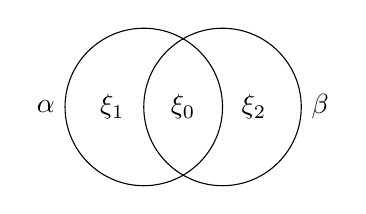
\begin{tikzpicture}
    \tikzstyle{circ}=[circle, draw, inner sep=0pt, minimum width=2cm]

    \node[circ, label=left:$\alpha$] (a) at (0,0) {}; 
    \node[circ, label=right:$\beta$] (b) at (1,0) {}; 
    \node at (-.4,0) {$\xi_1$};
    \node at (1.4,0) {$\xi_2$};
    \node at (.5,0)  {$\xi_0$};
    \end{tikzpicture}}
    \end{center}
\end{proof}

Давайте попробуем разобраться с аналогичным вопросом для троек случайных
величин. Энтропийный профиль для тройки $(\alpha,\beta,\gamma)$ будет задаваться 7 числами:
\[
\bigl(H(\alpha),H(\beta),H(\gamma),H(\alpha,\beta),H(\alpha,\gamma),
H(\beta,\gamma),H(\alpha,\beta,\gamma)\bigr).
\]
Для случайных величин $(\alpha,\beta,\gamma)$ можно записать 9 независимых
неравенств.
\begin{equation*}
\begin{array}{lll}
H(\alpha\mid\beta,\gamma)\ge 0, & I(\alpha:\beta )\ge 0, & I(\alpha:\beta\mid\gamma) \ge 0,\\
H(\beta\mid\gamma,\alpha)\ge 0, & I(\beta:\gamma )\ge 0, & I(\beta:\gamma\mid\alpha) \ge 0,\\
H(\gamma\mid\alpha,\beta)\ge 0, & I(\gamma:\alpha)\ge 0, & I(\gamma:\alpha\mid\beta) \ge 0.
\end{array}
\end{equation*}
\begin{definition}
Определим общую информацию трёх случайных величин
\[
    I(\alpha:\beta:\gamma) = I(\alpha:\beta) - I(\alpha:\beta\mid\gamma).
\]
\end{definition}

\begin{statement}
    Общая информация трёх случайных величин может быть отрицательной.
\end{statement}
\begin{proof}
    Пусть $\alpha$ и $\beta$ будут независимыми равномерно распределёнными на $\{0,1\}$ случайными
    величинами. Случайная величина $\gamma$ будет принимать значение из $\{0,1\}$ в соответствии со
    следующим соотношением:
    \[
        \alpha\oplus\beta\oplus\gamma = 0.
    \]
    Мы получим следующую картину:

    \begin{center}
    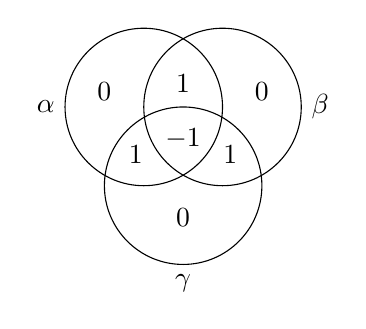
\begin{tikzpicture}
        \tikzstyle{circ}=[circle, draw, inner sep=0pt, minimum width=2cm]

        \node[circ, label=left:$\alpha$]  (a) at (1,1) {}; 
        \node[circ, label=right:$\beta$]  (b) at (2,1) {}; 
        \node[circ, label=below:$\gamma$] (c) at (1.5,0) {}; 
        \node at (0.5,1.2) {$0$};
        \node at (1.5,-.4) {$0$};
        \node at (2.5,1.2) {$0$};

        \node at (0.9,0.4) {$1$};
        \node at (1.5,1.3) {$1$};
        \node at (2.1,0.4) {$1$};

        \node at (1.5,0.6) {$-1$};
    \end{tikzpicture}
    \end{center}

\end{proof}
\begin{statement}
    Других неравенств для троек нет.
\end{statement}
\begin{statement}
        Есть профили, которые не реализуются никакими распределениями, но их мера 0.
\end{statement}
\begin{exercise}
    Доказать, что следующий профиль реализуется только при $h=\log n$ для некоторого целого $n$.
    \begin{center}
    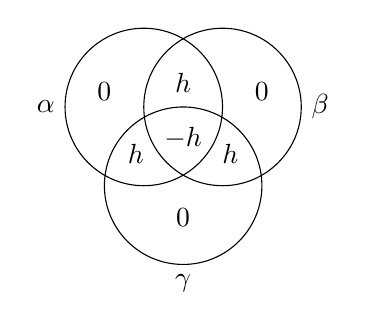
\begin{tikzpicture}
        \tikzstyle{circ}=[circle, draw, inner sep=0pt, minimum width=2cm]

        \node[circ, label=left:$\alpha$]  (a) at (1,1) {}; 
        \node[circ, label=right:$\beta$]  (b) at (2,1) {}; 
        \node[circ, label=below:$\gamma$] (c) at (1.5,0) {}; 
        \node at (0.5,1.2) {$0$};
        \node at (1.5,-.4) {$0$};
        \node at (2.5,1.2) {$0$};

        \node at (0.9,0.4) {$h$};
        \node at (1.5,1.3) {$h$};
        \node at (2.1,0.4) {$h$};

        \node at (1.5,0.6) {$-h$};
    \end{tikzpicture}
    \end{center}
\end{exercise}
\begin{statement}
    \(2H(\alpha,\beta,\gamma)\le H(\alpha,\beta) + H(\alpha,\gamma) + H(\beta,\gamma)\).
\end{statement}
\begin{corollary}[Теорема \ref{thm:volume}]
Для \(A\subset\bitstr\times\bitstr\times\bitstr\)
\[2\chi(A) \le \chi_{12}(A) + \chi_{13}(A) + \chi_{23}(A).\]
\end{corollary}
\begin{proof}
    Пусть $(\alpha,\beta,\gamma)$ равномерно распределены на $A$.
    \[
        2\chi(A) = 2H(\alpha,\beta,\gamma)\le 
        \underbrace{H(\alpha,\beta) }_{\le\chi_{12}(A)} + 
        \underbrace{H(\alpha,\gamma)}_{\le\chi_{13}(A)} + 
        \underbrace{H(\beta,\gamma) }_{\le\chi_{23}(A)}.
    \]
\end{proof}

\subsection{Неравенства о тройках}
Будем в различных предположениях доказывать следующее утверждение
\[
    H(a\mid x) + H(a\mid y) \le H(a).
\]

\begin{statement}
    Если $a,x,y$ такие, что
\[
    \begin{cases}
        H(a\mid y,x) = 0,\\
        I(x:y\mid a) = 0.
    \end{cases}
\]
то  \(H(a\mid x) + H(a\mid y) \le H(a)\).
\end{statement}
\begin{proof}
    Получается, что нам нужно доказать неотрицательность $h$. 
    \begin{center}
    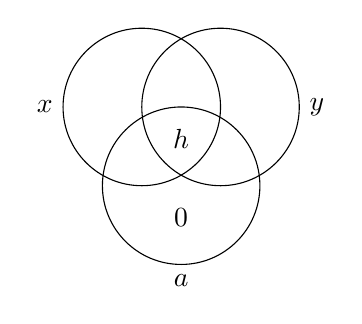
\begin{tikzpicture}
        \tikzstyle{circ}=[circle, draw, inner sep=0pt, minimum width=2cm]

        \node[circ, label=left:$x$]  (x) at (1,1) {}; 
        \node[circ, label=right:$y$] (y) at (2,1) {}; 
        \node[circ, label=below:$a$] (a) at (1.5,0) {}; 
        \node at (1.5,-.4) {$0$};

        \node at (1.5,0.6) {$h$};
    \end{tikzpicture}
    \end{center}
Т.к. $I(x:y\mid a) = 0$, то $h = I(x:y)\ge 0$.
\end{proof}
\begin{statement}
    Если $a,x,y$ такие, что $H(a\mid y,x) = 0$ и
\[
    \begin{cases}
        A_i \sim X_j\\
        A_i \sim Y_k
    \end{cases} \implies A_i\sim(X_i,Y_k),
\]
то  \(H(a\mid x) + H(a\mid y) \le H(a)\). (Обозначение $A_i\sim X_j$ $\iff$ $\Pr[a=A_i \land x=X_j]>0$.)
\end{statement}
\begin{remark}
    Условие $H(a\mid x,y) = 0$ можно интерпретировать так: $a = f(x,y)$.
\end{remark}
\begin{proof}
    Построим новое распределение $(a',x',y')$:
    \begin{itemize}
        \item $a'$ имеет то же распределение, что и $a$,
        \item условное распределение $x'$ при условии $a'$ совпадает
            с условным распределением $x$ при условии $a$,
        \item условное распределение $y'$ при условии $a'$ совпадает
            с условным распределением $y$ при условии $a$,
        \item $x'$ и $y'$ независимы при заданном $a'$.
    \end{itemize}
    \[\
    \Pr[a'=A_i, x' = X_j, y' = Y_k] = 
    \Pr[a'=A_i]\cdot \Pr[x' = X_j\mid a'=A_i]\cdot \Pr[y' = Y_k\mid a' = A_i].
    \]
    Таким образом
    \[
        H(a',x',y') = H(a') + H(x'\mid a') + H(y'\mid a') - \underbrace{I(x':y'\mid a')}_{0}.
    \]
    С другой стороны
    \[
        H(a',x',y') \le H(x') + H(y') + H(a'\mid x',y').
    \]
    Кроме того, мы может стереть штрихи почти везде.
    \[
        H(x) + H(y) + H(a'\mid x',y') \ge H(a',x',y') = H(a) + H(x\mid a) + H(y\mid a).
    \]
    Покажем, что $H(a'\mid x', y') = 0$, т.е. $a' = f(x',y')$. Действительно: 
    если тройка $(A_i, X_i, Y_k)$ в новом распределении встречается с положительной
    вероятностью, то и в исходном распределении она так же встречалась с положительной
    вероятностью, следовательно $a' = f(x',y')$.
    Получаем: $H(a) + H(x\mid a) + H(y\mid a) \le H(x) + H(y)$. Прибавим $H(a)$ к обеим частям
    неравенства:
    \[
       H(x,a) + H(y,a) \le H(x) + H(y) + H(a)\implies H(a\mid x) + H(a \mid y) \le H(a).
    \]
\end{proof}
\begin{problem}[Верещагин]
    Рассмотрим двудольный граф с вершинами $(L,R)$ с цветными рёбрами.
    Все рёбра инцидентные одной вершине разноцветные, степень в левой доле не меньше $n$, 
    в правой~--- не меньше $m$. Пусть известно, что для пары вершин $(x\in L, y\in R)$
    есть не более одного общего цвета. Докажите, что количество цветов хотя бы $n\cdot m$.

    Заметим, что одноцветные рёбра образуют паросочетания. Для каждого цвета $c$ соединим все
    согласованные с $c$ вершины слева с согласованными с $c$ вершинами справа. Получим биклику из
    рёбер цвета $c$.

    Рассмотрим распределение на тройках $(a,x,y)$ (цвет, вершина из левой доли, вершина из правой
    доли): выбираем цвет пропорционально размеру соответствующей биклики и выбираем случайное ребро
    этого цвета. Можно проверить, что выполняется следующее соотношение:
\[
    \begin{cases}
        A_i \sim X_j,\\
        A_i \sim Y_k,
    \end{cases} \implies A_i\sim(X_i,Y_k).
\]
Теперь применим: $\underbrace{H(a\mid x)}_{\ge\log n} + 
                  \underbrace{H(a\mid y)}_{\ge\log m} \le H(a) \le \log (\text{\# цветов})$.
\end{problem}

\section{Криптография}
\subsection{Шифрования с закрытым ключом}

Рассмотрим задачу кодирования сообщения при помощи симметричного шифрования.
Будем считать, что вычислительные ресурсы противника неограниченны. 
Предположим, что мы шифруем сообщение $x$ с ключом шифрования $k$. При
шифровании сообщения мы получаем \emph{шифрограмму} $m = E(x, k)$.
Получатель шифрограммы тоже знает ключ $k$ и может узнать исходное
сообщение $x= D(m,k).$

Будем предполагать, что $x$ и $k$ являются случайными 
величинами. Противник не знает $x$ и $k$, но знает $m$. Для идеальной
схемы шифрования должны выполняться следующие соотношения:
\[
\begin{cases}
    H(m\mid x,k) = 0,\\
    H(x\mid m,k) = 0,\\
    I(m : x) = 0.
\end{cases}
\]

\begin{theorem}[Шеннон]
    $H(k)\ge H(m)$, даже если мы ослабим условие выкинув первое условие
    $H(m\mid x,k) = 0$ (т.е. разрешим алгоритму $E$ использовать случайные
    биты).
\end{theorem}     
\begin{remark}
    Одноразовый блокнот (one-time notepad) обладает этим свойством.
\end{remark}
\begin{proof}
    По условию $a + d = 0$, т.е. $d = -a$. 

    \begin{center}
    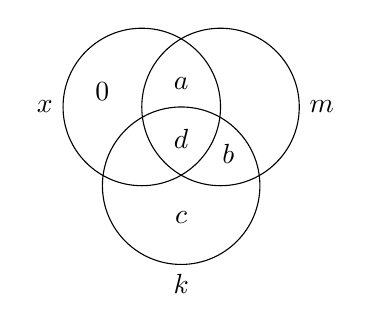
\begin{tikzpicture}
        \tikzstyle{circ}=[circle, draw, inner sep=0pt, minimum width=2cm]

        \node[circ, label=left:$x$]  (a) at (1,1) {}; 
        \node[circ, label=right:$m$]  (b) at (2,1) {}; 
        \node[circ, label=below:$k$] (c) at (1.5,0) {}; 
        \node at (0.5,1.2) {$0$};
        \node at (1.5,-.4) {$c$};

        \node at (1.5,1.3) {$a$};
        \node at (2.1,0.4) {$b$};

        \node at (1.5,0.6) {$d$};
    \end{tikzpicture}
    \end{center}
    Т.к. взаимная информация неотрицательна, то $d + b\ge 0$, т.е. 
    $b \ge -d = a$. Теперь из $b \ge a$ и $c\ge 0$ следует $H(k)\ge H(x)$.                                  
\end{proof}


\subsection{Схемы разделения секрета}

Пусть у нас есть некоторый секрет $S_0$ и $n$ участников и мы хотим разделить между ними этот секрет
так, чтобы они могли им воспользоваться только все вместе, а любое подмножество участников~--- не
могло.
\begin{definition}
    \emph{Совершенная схема разделения секрета}~--- это совместное распределение вероятностей
    $(S_0,\seqn{S}{n})$, такое что
    \[
    \begin{cases}
        H(S_0\mid\seqn{S}{n}) = 0,\\
        H(S_0\mid\seqin{S}{i}{k}) = H(S_0), & k <  n.
    \end{cases}
    \]
    Второе условие можно переписать как $I(S_0:\seqin{S}{i}{k}) = 0$.
\end{definition}

Для совершенной схемы разделения секрета есть простая конструкция. Будем считать, что $S_0$
записан (закодирован) при помощи $\ell$ бит. Выберем независимо и равномерно
$S_1,\dotsc,S_{n-1}\in\{0,1\}^\ell$. $S_n$ определяется из условия 
$S_0 \oplus S_1 \oplus S_2 \oplus \dotsb \oplus S_n = \vec 0$ (покоординатная сумма по модулю 2).
\begin{statement}
    Предложенная схема разделения секрета является совершенной.
\end{statement}

\begin{definition}
    \emph{Пороговая совершенная схема разделения секрета}~--- это совместное распределение вероятностей
    $(S_0,\seqn{S}{n})$, такое что
    \[
    \begin{cases}
        H(S_0\mid\seqin{S}{i}{t}) = 0,\\
        H(S_0\mid\seqin{S}{i}{k}) = H(S_0), & k < t.
    \end{cases}
    \]
\end{definition}
\paragraph{Пороговая схема Шамира.} Будем считать, что секрет $S_0$~--- это элемент некоторого конечного
поля $\mathbb{F}_q$. Выберем случайный многочлен $p$ над полем $\mathbb{F}_q$ степени не более
$t-1$: выберем $t-1$ коэффициент независимо и равномерно, а последний (свободный) коэффициент определим из
соотношения $p(0) = S_0$. Выберем произвольным образом и сообщим всем участникам некоторый
набор различных ненулевых элементов поля $\seqn{a}{n}\in\mathbb{F}_q$ и вычислим секреты участников
как значение полинома в соответствующих точках $S_i = p(a_i)$. Теперь любые $t$ участником могут
собраться, воспользоваться формулой для интерполяции многочлена и вычислить $S_0=p(0)$. Если же
соберётся меньше участников, то у них не будет никакой информации об $S_0$.
\begin{statement}
    Пороговая схема Шамира является совершенной.
\end{statement}
\begin{proof}
    Любой полином степени меньше $t-1$ можно дополнить до полинома большей степени с любым значением в точке $0$.
\end{proof}

\begin{definition}
    \emph{Совершенная схема разделения секрета для структуры доступа $\Gamma\subset
    2^{[n]}$} ($\Gamma$ должно быть замкнуто вверх)~--- это совместное распределение вероятностей
    $(S_0,\seqn{S}{n})$, такое что
    \[
    \begin{cases}
        H(S_0\mid\seqin{S}{i}{m}) = 0,      & \{\seqn{i}{m}\}\in\Gamma,\\
        H(S_0\mid\seqin{S}{i}{m}) = H(S_0), & \{\seqn{i}{m}\}\not\in\Gamma.
    \end{cases}
    \]
\end{definition}
\begin{definition}
    \emph{Идеальная схема разделения секрета}~--- это
    совершенная схема разделения секрета с дополнительным требованием ,,экономности``.
    \[
    \forall i\in\{1,2,\dotsc,n\},\ H(S_i)\le H(S_0).
    \]
\end{definition}

\begin{statement}
        Если участник $i$ является \emph{существенным} в структуре доступа $\Gamma$ (т.е. существует
        такое $s\in\Gamma$, что $s\setminus\{i\}\not\in\Gamma$), то $H(S_i)\ge H(S_0)$. 
\end{statement}
\begin{remark}
    Схема Шамира является идеальной.
\end{remark}
\begin{proof} Пусть $s=\{i,\seqn{j}{k}\}\in\Gamma$, а $s\setminus \{i\}\not\in\Gamma$. 
    Обозначим взаимную информацию  $I(S_0:\seqin{S}{j}{k}\mid S_i)$ за $h$, 
    а $I(S_i:\seqin{S}{j}{k}\mid S_0)$ за $g$. Из условия 
    $I(S_0:\seqin{S}{j}{k}) = 0$ получаем, что $I(S_0:S_i:\seqin{S}{j}{k}) = -h$, аналогичным
    образом из $I(S_i:\seqin{S}{j}{k})\ge 0$ получаем, что $g \ge h$.

    \begin{center}
    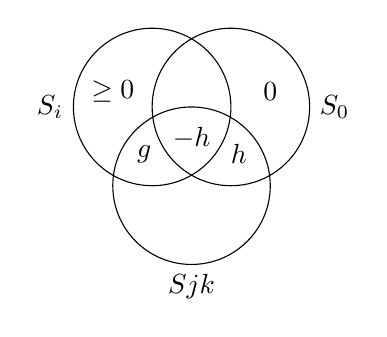
\begin{tikzpicture}
        \tikzstyle{circ}=[circle, draw, inner sep=0pt, minimum width=2cm]

        \node[circ, label=left:$S_i$]  (a) at (1,1) {}; 
        \node[circ, label=right:$S_0$]  (b) at (2,1) {}; 
        \node[circ, label=below:$\seqin{S}{j}{k}$] (c) at (1.5,0) {}; 
        \node at (0.5,1.2) {$\ge 0$};
        \node at (2.5,1.2) {$0$};

        \node at (2.1,0.4) {$h$};
        \node at (0.9,0.4) {$g$};

        \node at (1.5,0.6) {$-h$};
    \end{tikzpicture}
    \end{center}
    Таким образом $H(S_i) \ge H(S_0)$.
\end{proof}
\begin{remark}
    Это утверждение показывает, что не бывает более ,,экономной`` схемы разделения секрета, чем идеальная.
\end{remark}


\begin{statement}
    Для любой системы доступа $\Gamma$ существует совершенная схема разделения секрета.
\end{statement}
\begin{proof}
    Давайте для каждого подмножества $A = \{\seqn{i}{k}\}\in\Gamma$ создадим собственный набор секретов
    $S^A_{i_1}, S^A_{i_2},\dotsc,S^A_{i_k}$: $S^A_{i_1}\oplus S^A_{i_2}\oplus\dotsb\oplus S^A_{i_k}
    = S_0$. 
   (Достаточно рассматривать только минимальные множества $A$.)
\end{proof}
\begin{remark}
    Предложенная схема не является идеальной.
\end{remark}

\begin{statement}
    Существуют структуры доступа, для которых не существует идеальной схемы разделения секрета.
\end{statement}
\begin{proof}
    Рассмотрим структуру доступа, заданную следующим графом (рёбра соответствуют авторизованным
    множествам).
    \begin{center}
    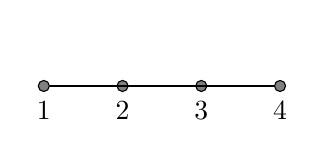
\begin{tikzpicture}
    \tikzstyle{vert}=[circle, draw, fill=black!50,
                            inner sep=0pt, minimum width=4pt]
    \node[vert, label=below:1, label=above:\strut] (a) at (1,0) {}; 
    \node[vert, label=below:2] (b) at (2,0) {};
    \node[vert, label=below:3] (c) at (3,0) {};
    \node[vert, label=below:4] (d) at (4,0) {};

    \path (a) edge (b) edge (c) edge (d);
    \end{tikzpicture}
    \end{center}
    Покажем, что для этой структуры доступа $H(S_2) + H(S_3) \ge 3H(S_0)$, другими словами
    $\max_i\frac{H(S_i)}{H(S_0)} \ge 3/2$.

    Для доказательства нам потребуются три леммы. Будем обозначать $h = H(S_0)$.
    \begin{lemma}
        $H(S_2\mid S_1, S_3) \ge h$.
    \end{lemma}
    \begin{proof} Второй участник может восстановить секрет, воспользовавшись либо секретом первого
        или секретом третьего участника, т.е. $I(S_2 : S_0 \mid S_1, S_3) = h$.
    \begin{center}
    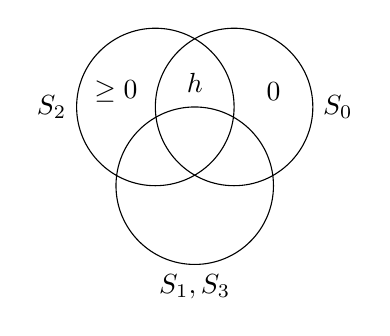
\begin{tikzpicture}
        \tikzstyle{circ}=[circle, draw, inner sep=0pt, minimum width=2cm]

        \node[circ, label=left:$S_2$]  (a) at (1,1) {}; 
        \node[circ, label=right:$S_0$]  (b) at (2,1) {}; 
        \node[circ, label=below:{$S_1,S_3$}] (c) at (1.5,0) {}; 
        \node at (0.5,1.2) {$\ge 0$};
        \node at (2.5,1.2) {$0$};
        \node at (1.5,1.3) {$h$};
    \end{tikzpicture}
    \end{center}
    Таким образом $H(S_2 \mid S_0) \ge  I(S_2:S_0\mid S_1,S_3) = h$.
    \end{proof}

    \begin{lemma}
        $H(S_3\mid S_1) \ge h$.
    \end{lemma}
    \begin{proof} Аналогично предыдущей лемме получаем, что $H(S_3\mid S_1, S_4)\ge h$, и как
        следствие $H(S_3\mid S_1)\ge h$.
    \begin{center}
    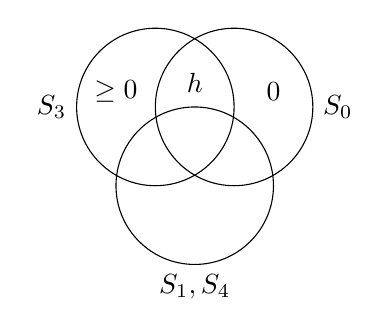
\begin{tikzpicture}
        \tikzstyle{circ}=[circle, draw, inner sep=0pt, minimum width=2cm]

        \node[circ, label=left:$S_3$]  (a) at (1,1) {}; 
        \node[circ, label=right:$S_0$]  (b) at (2,1) {}; 
        \node[circ, label=below:{$S_1,S_4$}] (c) at (1.5,0) {}; 
        \node at (0.5,1.2) {$\ge 0$};
        \node at (2.5,1.2) {$0$};
        \node at (1.5,1.3) {$h$};
    \end{tikzpicture}
    \end{center}
    \end{proof}

    \begin{lemma}\label{lm:secret4:l3}
        $I(S_1 : S_3\mid S_2) \ge h$.
    \end{lemma}
    \begin{proof} 
        Следующую схему следует интерпретировать как энтропия при условии $S_2$.
    \begin{center}
    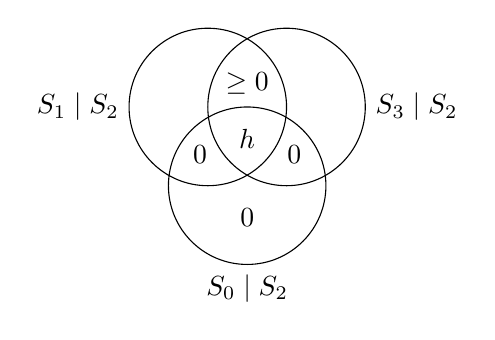
\begin{tikzpicture}
        \tikzstyle{circ}=[circle, draw, inner sep=0pt, minimum width=2cm]

        \node[circ, label=left: $S_1\mid S_2$]  (a) at (1,1) {}; 
        \node[circ, label=right:$S_3\mid S_2$]  (b) at (2,1) {}; 
        \node[circ, label=below:$S_0\mid S_2$] (c) at (1.5,0) {}; 

        \node at (0.9,0.4) {$0$};
        \node at (1.5,1.3) {$\ge0$};
        \node at (2.1,0.4) {$0$};

        \node at (1.5,-.4) {$0$};
        \node at (1.5,0.6) {$h$};
    \end{tikzpicture}
    \end{center}
    Заметим, что $I(S_1 : S_0 \mid S_2) = h$ и $I(S_3 : S_0 \mid S_2) = h$ в то время, 
    как $I(S_1 : S_0 \mid S_2, S_3) = 0$ и $I(S_3 : S_0 \mid S_1, S_2) = 0$.
    Т.е. $I(S_1:S_3:S_0\mid S_2) = h$, следовательно $I(S_1 : S_3\mid S_2) \ge h$.
    \end{proof}
    Теперь осталось сложить результаты трёх лемм: 
    \[
        H(S_2) + H(S_3)\ge H(S_2,S_3) = H(S_2\mid S_1,S_2) + H(S_3\mid S_1) + I(S_1:S_3\mid S_2) +
        I(S_2:S_1) \ge 3h.
    \]
\end{proof}
\begin{exercise}
    Доказать, что для любой схемы разделения секреты для этой структуры
    $\max_i\frac{H(S_i)}{H(S_0)} \ge 3/2$.
    \begin{center}
    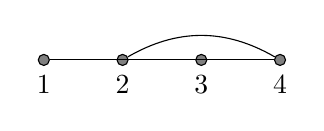
\begin{tikzpicture}
    \tikzstyle{vert}=[circle, draw, fill=black!50,
                            inner sep=0pt, minimum width=4pt]
    \node[vert, label=below:1] (a) at (1,0) {}; 
    \node[vert, label=below:2] (b) at (2,0) {};
    \node[vert, label=below:3] (c) at (3,0) {};
    \node[vert, label=below:4] (d) at (4,0) {};

    \path (a) edge (b) edge (c) edge (d)
          (b) edge[bend left] (d);
    \end{tikzpicture}
    \end{center}
\end{exercise}
\begin{theorem}[Csirmaz'94]
    Существуют структуры доступа $\Gamma$ на $n$ участниках, такие что для любой схемы разделения
    секрета $\max_i\frac{H(S_i)}{H(S_0)} \ge \Omega(n/\log n)$.
\end{theorem}
\begin{proof}
    Выберем $n$ и $k$ такие, что $n = 2^k + k + 1$, и два множества участников 
    \[
        \begin{array}{l}
            A = \{\seqn{a}{k}\},\\
            B = \{\seqn{b}{2^k - 1}\}.
        \end{array}
    \]
    Для определения структуры доступа нам потребуются два семейства множеств. 
    Пусть $\{A_0,\seqn{A}{2^k-1}\}$~--- это все подмножества $A$, причём $A_0 = A$ и для любых
    $i < j$ выполняется $A_i\not\subseteq A_j$ (например, можно их упорядочить по уменьшению
    размера). Построим множества $\{B_0,\seqn{B}{2^k - 1}\}$ следующим образом: $B_0 = \emptyset$, 
    $B_i = \{\seqn{b}{i}\}$.  
    Теперь мы готовы определить структуру доступа $\Gamma$: $\Gamma = \{U_i\}_{i=0}^{2^k-1}$, где $U_i =
    A_i\cup B_i$. 
    
    Как и в предыдущих утверждениях обозначим $H(S_0)$ за $h$.
    В дальнейших рассуждениях мы будем использовать следующую нотацию: под энтропией некоторого
    множества участников $X = \{\seqn{x}{t}\}\subset A\cup B$, мы будем понимать энтропию секретов, которые
    принадлежат участникам этого множества, т.е. $H(X) = H(\seqin{S}{x}{t})$.

    \begin{lemma}\label{lm:secretlb} Для $i=\{0,1,2,\dots,2^k-2\}$
        \[
            H(A\cup B_i) - H(B_i) \ge H(A\cup B_{i+1}) - H(B_i+1) + h.
        \]
    \end{lemma}
    Из этой леммы следует, что 
    \begin{multline*}
        H(A) = H(A\cup B_0) - H(B_0) \ge H(A\cup B_{1}) - H(B_1) + h \ge \dotsb \ge\\
        \ge \underbrace{H(A\cup B_{2^k-1}) - H(B_{2^k-1})}_{\ge 0} + (2^k - 1)\cdot h.
    \end{multline*}
    Получаем, что $H(A) = H(\seqin{S}{a}{k})\ge (2^k - 1) \cdot h$. Следовательно есть $i$ такое,
    что $H(S_{a_i})\ge \frac{2^k - 1}{k}\cdot h$.
    Вспомним, что мы выбрали $n = 2^k + k + 1$, т.е. $H(S_{a_i})\ge \Omega(n/\log n) \cdot h$.
    Осталось доказать лемму.
    \begin{proof}[Доказательство леммы \ref{lm:secretlb}]
        Докажем два неравенства:
        \begin{enumerate}
            \item $H(A_{i+1}\cup B_i) + H(B_{i+1}) \ge  H(A_{i+1} \cup B_{i+1}) + H(B_i) $.
            \item $H(A\cup B_i) + H(A_{i+1}\cup B_{i+1}) \ge H(A\cup B_{i+1}) + H(A_{i+1}\cup B_i) + h$.
        \end{enumerate}
%        Заметим, что если сложить эти два неравенства, то мы получим утверждение леммы.
%    
%        Первое неравенства говорит о неотрицательности условной совместной информации.
%        Действительно, давайте вспомним формулу для условной совместной информации:
%        \[
%            I(x:y\mid z) \ge 0 \iff H(x,z) + H(y,z)\ge H(x,y,z) + H(z).
%        \]
%        Таким образом первое неравенство утверждает $I(A_{i+1}:\{b_{i+1}\}\mid B_i)\ge 0$.
%
%        Аналогично второе неравенство утверждает, $I(A:\{b_{i+1}\}\mid A_{i+1}\cup B_i)\ge h$.
%        Доказательство этого утверждения аналогично лемме~\ref{lm:secret4:l3}~--- нужно рассмотреть
%        условное распределение при известном $A_{i+1}\cup B_i$.
%    \begin{center}
%    \begin{tikzpicture}
%        \tikzstyle{circ}=[circle, draw, inner sep=0pt, minimum width=2cm]
%
%        \node[circ, label=left:$A\mid A_{i+1}\cup B_i$]  (a) at (1,1) {}; 
%        \node[circ, label=right:{$\{b_{i+1}\}\mid A_{i+1}\cup B_i$}]  (b) at (2,1) {}; 
%        \node[circ, label=below:{$S_0\mid A_{i+1}\cup B_i$}] (c) at (1.5,0) {}; 
%        \node at (0.9,0.4) {$0$};
%        \node at (1.5,1.3) {$\ge0$};
%        \node at (2.1,0.4) {$0$};
%
%        \node at (1.5,-.4) {$0$};
%        \node at (1.5,0.6) {$h$};
%    \end{tikzpicture}
%    \end{center}
    \end{proof}
    Эта лемма завершает доказательство теоремы.
\end{proof}
    \begin{remark}
        Нижние оценки на избыточную сложность совершенных схем разделения
        секрета влекут нижние оценки на схемную сложность монотонных функций.
    \end{remark}

\section{Коммуникационная сложность}
Пусть $X$, $Y$ и $Z$~--- это три конечных множества, и пусть задана некоторая функция $f:X\times Y \to Z$.
Два игрока, будем называть их Алиса и Боб, решают \emph{коммуникационную задачу для функции $f$}, если:
\begin{enumerate}
    \item множества $X$, $Y$, $Z$ и функция $f$ известны обоим игрокам,
    \item Алиса знает некоторое $x\in X$,
    \item Боб знает некоторое $y\in Y$,
    \item Алиса и Боб стремятся вычислить $f(x,y)$.
\end{enumerate}
Для решения этой коммуникационной задачи Алиса и Боб могут пересылать друг другу сообщения.
Задача считается решённой, если оба игрока знают $f(x,y)$.
Нас интересует минимальное количество битов, которое необходимо и достаточно переслать
для вычисления $f(x,y)$.

\begin{definition}
\emph{Коммуникационный протокол} для функции $f: X\times Y \to Z$~--- это корневое
двоичное дерево, которое описывает совместное вычисление Алисой и Бобом функции $f$.
В этом дереве каждая внутренняя вершина $v$ помечена меткой А или Б,
означающей очередь хода Алисы или Боба соответственно.
Для каждой вершины, помеченной А, определена функция $g_v: X \to \bits$, 
которая говорит Алисе, какой бит нужно послать,
если вычисление находится в этой вершине. Аналогично, для каждой вершины $v$ 
с пометкой Б определена функция $h_v: Y\to \bits$, которая определяет бит, 
который Боб должен отослать в этой вершине. Каждая внутренняя вершина имеет двух
потомков, ребро к первому потомку помечено $0$, а ребро ко второму потомку
помечено $1$. Каждый лист помечен значением из множества $Z$.

Вычисление по такому протоколу на конкретной паре входов $(x,y)$ устроено так:
изначально вычисление находится в корне. В каждой внутренней вершине $v$ в 
зависимости от пометки либо Алиса, либо Боб пересылают один бит 
(он определяется соответствующей функцией $g_v$ или $h_v$). После этого
вычисление переходит в один из потомков вершины $v$ по ребру, пометка которого
совпадает с битом, переданным в вершине $v$. Когда вычисление приходит в лист,
то оно завершается. Результат вычисления~--- это пометка в листе.
\end{definition}

Будем говорить, что коммуникационный протокол \emph{вычисляет функцию $f$}, если
для всех пар $(x,y)\in X\times Y$ вычисление приходит в лист с пометкой $f(x,y)$.
Теперь можно дать формальное определение \emph{коммуникационной сложности функции $f$}.

Аналогичным образом можно определить \emph{коммуникационный протокол, вычисляющий отношение $R \subset (X\times
Y)\times Z$}~--- нужно только дополнительно потребовать, чтобы ответы Алисы и Боба были согласованы.

\begin{definition} 
    \emph{Коммуникационная сложность} функции $f$ определяется как наименьшая глубина
    протокола (максимальная рёберная длина пути от корня до листа), вычисляющего функцию $f$.
    Обозначается $D(f)$.
\end{definition}

\begin{statement}
        Для любой $f: \{0,1\}^n \times\{0,1\}^n \to \bits$, $D(f) \le n + 1$.
\end{statement}
\begin{proof}
        Алиса посылает Бобу свой вход, а Боб посылает Алисе значение $f$.
\end{proof}

\begin{example} Примеры функций с нетривиальной верхней оценкой на коммуникационную сложность.
    \begin{enumerate}
        \item (Pointer Chaising) $D(\mathrm{PC})\le k\log n$, 
            где $PC(x,y) = \underbrace{x(y(x(y(x(y(x(y(x}_{\text{$k$ раундов}}(0)))))))))$.
            У игроков есть двудольный ориентированный граф на $2n$ вершинах, у которого исходящая
            степень каждой вершины равна 1. Алиса знает левую долю, Боб~--- правую.
            В начале они кладут фишку на вершину с номером 0 из доли Алисы и начинают
            передвигать её по рёбрам. Всего они должны сделать  $k$ переходов по рёбрам графа.
            Ответ~--- номер финальной вершины.


        \item $D(\mathrm{MED}) = O(\log^2 n)$, где $x$ и $y$ интерпретируются как характеристические
            функции подмножеств $[n]$, а $\mathrm{MED}(x,y)$~--- медиана их объединения.
        \item $D(CIS_G) = O(\log^2 n)$, где $x$ интерпретируется как характеристическая
            функция некоторой клики в графе $G$, а $y$~--- как характеристическая 
            функция некоторого независимого множества в графе $G$. $\mathrm{CIS}(x,y) = 1$, 
            если клика и независимое множество имеют общую вершину.
            (Замечание: не известно графов $G$, для которых нельзя решить 
            эту задачу за $O(\log n)$.)
    \end{enumerate}
\end{example}

\subsection{Нижние оценки}
    Рассмотрим коммуникационный протокол для некоторой функции $f: X\times Y\to Z$. 
    Для каждой вершины $v$ определим множество $R_v\subset X\times Y$~--- множество
    всех пар $(x,y)\in X\times Y$, для которых вычисление приходит в вершину $v$.
\begin{statement}
    Для всех вершин $v$ множество $R_v$ является комбинаторным прямоугольником,
    т.е. существуют такие $X_v\subset X$ и $Y_v\subset Y$, что $R_v = X_v\times Y_v$.
\end{statement}
\begin{proof}
    Покажем по индукции. Это верно для корня. Если это верно для какой-то вершины $v$
    с пометкой А: $R_v = X_v\times Y_v$. Если Алиса пересылает бит $b$ и вычисление
    переходит в вершину $u$, то $R_u = X_u\times Y_u$, 
    где $X_u = \{x\in X_v\mid g_v(x) = b\}$, а $Y_u = Y_v$. Аналогично, если Боб 
    посылает бит $b$ и вычисление переходит в вершину $u$, то $R_u = X_u\times Y_u$, 
    где $X_u = X_v$, а $Y_u = \{y\in Y_v\mid h_v(y) = b\}$.
\end{proof}
\begin{corollary}
    Листья коммуникационного протокола для функции $f$ задают разбиение множества $X\times Y$ на 
    одноцветные прямоугольники.
\end{corollary}

Будем обозначать $C^R(f)$~--- минимальное количество \emph{одноцветных} прямоугольников, покрывающих $X\times Y$.

\begin{statement}
    $D(f) \ge \log C^R(f)$.
\end{statement}
\begin{proof}
    $D(f) \ge \log (\text{\# листьев}) \ge \log C^R(f)$.
\end{proof}


\paragraph{Метод размера прямоугольников.} Определим некоторую весовую функцию на элементах $X\times Y$.
Тогда верна следующая оценка \[
    C^R(f) \ge \frac{w(X\times Y)}{\max\limits_{\text{одноцв. } A\times B} w(A\times B)}. 
\]


\paragraph{Метод трудного множества (fooling set).} Это частный случай метода размера прямоугольников, 
при котором фиксируется некоторое множество $F\subset X\times Y$, а $w(x,y)$ определяется следующим образом:
\[
    w(x,y) = 
    \begin{cases}
        1, & (x,y)\in F,\\
        0, & (x,y)\not\in F.
    \end{cases}
\]
При этом никакой прямоугольник не содержит более одного элемента из $F$. Следовательно $C^R(f) \ge |F|$.

\paragraph{Метод ранга матрицы.} Рассмотрим \emph{матрицу функции $f$}~--- матрицу, в которой
строки индексированы элементами $X$, столбцы~--- элементами $Y$, а в ячейке $(x,y)$ стоит $f(x,y)$.
Если мы рассмотрим эту матрицу функции как матрицу $M$ над некоторым довольно большим полем, 
то можно показать, что $C^R(f)\ge \rank M$.
\begin{exercise}
    Докажите предыдущие утверждения.
\end{exercise}

\begin{statement}
    $D(\mathrm{EQ}) = n + 1$, где $\mathrm{EQ}(x,y) = 1 \iff x = y$.
\end{statement}

\begin{statement}
    $D(\mathrm{GE}) = n + 1$, где $\mathrm{GE}(x,y) = 1 \iff x \ge y$.
\end{statement}


\subsection{Связь протоколов и формул}
\begin{definition}  
    \emph{Игра Карчмера-Вигдерсона для функции $f : \{0,1\}^n \to \{0,1\}$}~--- это 
    следующая коммуникационная игра: Алиса получает $x\in f^{-1}(0)$, Боб получает 
    $y\in f^{-1}(1)$, и они вместе пытаются найте такое $i\in [n]$, что $x_i \neq y_i$. 
    Другими словами, игра Карчмера-Вигдерсона~--- это коммуникационная задача для 
    \emph{отношения} $$R_f = \{((x,y),i)\mid x\in f^{-1}(0), y\in f^{-1}(1), x_i\neq y_i\}.$$
    Отношение $R_f$ будем называть \emph{отношением Карчмера-Вигдерсона} для функции $f$.
\end{definition}

\begin{definition}
    \emph{Формула в базисе Де Моргана для функции $f:\{0,1\}^n \to \{0,1\}$}~--- это булевая 
    формула с переменными $\{\seqn{x}{n}\}$, соответствующим отдельным битам входа $f$,
    и со связками $\{\land, \lor, \neg\}$, вычисляющая функцию $f$.
    Законы Де Моргана позволяют нам предполагать, что все $\neg$ находятся непосредственно
    перед переменными. Заметим, что структура формулы Де Моргана представляет собой корневое дерево
    (листья соответствуют переменным, а внутренние вершина~--- логическим связкам).
\end{definition}

Будем называть \emph{формульной сложностью} $L(f)$ функции $f : \{0,1\}^n \to \{0,1\}$ ~---
это размер (количество вхождений переменных) минимальной формулы вычисляющей $f$. Если
говорить более формально, то нужно говорить не о конкретной функции, а о последовательности
функций.

\begin{definition}
    Для функции $f:\bitstr\to\{0,1\}$ определим последовательность функций $\{\seqn{f}{n},\dotsc\}$,
    где $f_i: \{0,1\}^i\to\{0,1\}$ и $\forall x\in\{0,1\}^i, f(x) = f_i(x)$. Тогда формульная сложность
    $L(f)$ функции $f$ ограничена $g(n)$, если для любого $n$ существует формула $\phi_n$ размера
    не более $g(n)$, вычисляющая функцию $f_n$.
\end{definition}

\begin{theorem}[Шеннон]
    Существует $f$: $L(f) = \Omega(2^n/n)$.
\end{theorem}
\begin{proof}
    Посчитаем количество формул размера не более $s$ (будем предполагать, что $s\ge n)$: 
    это количество можно оценить сверху как $(4\cdot s)^s$. В то же время число всех функций 
    $f: \{0,1\}^n \to \{0,1\}$ ровно $2^{2^n}$. Какого $s$ достаточно,
    чтобы вычислить все функции на $n$ битах?
    $$(4\cdot s)^s \ge 2^{2^n} \implies s\cdot \log(4\cdot s) \ge 2^n \implies s = \Omega(2^n/n).$$
\end{proof}
\begin{remark}
    Этот подсчёт показывает, что существуют функции с экспоненциальной формульной сложностью.
    Более того, любая случайная функция с большой вероятностью имеет такую сложность.
\end{remark}

Однако не известно \emph{явных} функций большой сложности. Лучшая известная на данный момент
нижняя оценка на формульную сложность явной функции это $\Omega(n^3)$ 
(оценка для функции Андреева, доказана Хостадом).

\begin{theorem}[Карчмер-Вигдерсон]
    Для каждой формулы $\phi$ вычисляющей $f$, существует такой
    протокол $\Pi_\phi$ для отношения Карчмера-Вигдерсона $R_f$, что его дерево
    совпадает с деревом, описывающим структуру формулу $\phi$. 
    Верно и обратное утверждение: если есть протокол для $R_f$, 
    то есть и формула с такой же структурой.
\end{theorem}
\begin{proof}
    Ход Алисы будет соответствовать связке $\land$,
    ход Боба~--- связке $\lor$. 

    \begin{itemize}
        \item \textbf{формула $\to$ протокол}\\
            Каждая внутренняя вершина протокола соответствует некоторой
            подформуле исходной формулы $\phi$. Будем поддерживать следующий инвариант: пусть $\phi_v$~--- 
            подформула, соответствующая текущей вершине протокола $v$, тогда $\phi_v(x) = 0$, а $\phi_v(y) = 1$.
            Это верно для начальной вершины (т.к. верно для $\phi$). Если для текущей вершины это верно, и
            $\phi_v = \phi_{v0} \land \phi_{v1}$, то Алиса пересылает бит $b$ такой, что
            $\phi_{vb}(x) = 0$ (такой бит должен быть по свойствам $\land$, т.к. $\phi_v(x) = 0$). 
            При этом мы знаем, что $\phi_v(y) = \phi_{v0}(y) = \phi_{v1}(y) = 1$, т.е. инвариант сохраняется.
            Аналогично, если $\phi_v = \phi_{v0} \lor \phi_{v1}$, то Боб пересылает бит $b$ такой, 
            что $\phi_{vb}(y) = 1$ (мы соответственно знаем, что $\phi_v(x) = \phi_{v0}(x) = \phi_{v1}(x) = 1$).
            Когда Алиса и Боб придут в некоторый лист, то по индукции получается, что значение в этом 
            листе на входе Алисы отличается от значения в листе на входе Боба, а значит номер переменной
            в листе соответствует номеру бита различия.

        \item \textbf{протокол $\to$ формула}\\
            Будем последовательно строить формулы для внутренних вершин протокола от листьев к корню.
            При этом будем поддерживать следующий инвариант: пусть $v$~--- вершина протокола, $X_v\times Y_v$~---
            соответствующий прямоугольник, тогда формула $\phi_v$ для вершины $v$ такая, что для всех $x\in X_v$,
            $\phi_v(x) = 0$ и для всех $y\in Y_v$, $\phi_v(y) = 1$. Пусть мы построили формулы $\phi_{v0}$ и
            $\phi_{v1}$ для сыновей некоторой вершины $v$. Если вершина $v$ соответствовала ходу Алисы,
            то для всех входов Алисы из множества $X_v$ формула $\phi_v$ должна быть равна 0. При 
            этом по индукционному предположению мы знаем, что для некоторых входов Алисы (на которых Алиса 
            посылает 0) $\phi_{v0}=0$, а для остальных обязательно $\phi_{v1} = 0$. С другой стороны для всех 
            входов Боба $y\in Y_v$, $\phi_{v0}(y) = \phi_{v1}(y) = 1$. Поэтому, если мы положим 
            $\phi_v = \phi_{v0} \land \phi_{v1}$, то инвариант сохранится. Аналогично, если вершина
            соответствовала ходу Боба, то следует положить $\phi_v = \phi_{v0} \lor \phi_{v1}$.

            Осталось объяснить, что мы будем делать с листьями. Заметим, что если в листе протокола
            написан некоторый индекс $i$, то в него могут попадать либо пары входов, для которых 
            ($x_i = 0$, $y_i=1$), либо входы, для которых ($x_i=1$, $y_i=0$), но не могут попадать
            одновременно. В противном случае можно было бы воспользоваться свойствами 
            комбинаторных прямоугольников и дать Алисе и Бобу входы с одинаковыми $i$-ми битами,
            которые привели бы в этот же лист.
            $$\begin{cases}
                (x,y)\in R_\ell, & x_i = 0, y_i = 1,\\
                (x',y')\in R_\ell, & x'_i = 1, y'_i = 0.
              \end{cases} \implies (x', y) \in R_\ell.
            $$
            Таким образом можно считать, что в каждом листе кроме номера бита различия записаны
            также значения этого бита у Алисы и у Боба. Если в листе $\ell$ с номером бита различия $i$
            записаны ($x_i = 0$, $y_i = 1$), то $\phi_\ell = x_i$, в обратном случае
            $\phi_\ell = \neg x_i$. 
    \end{itemize}
\end{proof}

Таким образом мы получили взаимно однозначное соответствие между протоколами и формулами.
Проблема в том, что сложность протоколов мы до этого измеряли в терминах максимальной 
глубины, а сложность формул~--- в терминах количества листьев. Давайте определим сложность
протокола в терминах количества листьев.

\begin{definition}
    Для отношения $R_f$ будем обозначать через $L(R_f)$ минимальное количество
    листьев в коммуникационном протоколе для $R_f$.
\end{definition}

\begin{corollary}
    Для любой функции $f$, $L(f) = L(R_f)$.
\end{corollary}

%С некоторыми потерями можно связать минимальный размер формулы для $f$ с минимальной глубиной формулы для $f$.
%\begin{statement}
%    Для любой $\alpha > 1$  и для любой формулы $\phi$ размера $s$ существует эквивалентная
%    формула $\phi'$ размера $s^\alpha$ и глубины $O(\log s)$ (константа зависит от $\alpha$).
%\end{statement}
%\begin{proof}
%    Определим рекурсивный алгоритм $A(\phi)$:
%    найдём в $\phi$ подформулу $\psi$ размера от $s/3$ до $2s/3$. 
%    Вернём $\phi' = (A(\psi) \land A(\phi|_{\psi = 1}))\lor(\neg A(\psi) \land A(\phi|_{\psi = 0})).$
%    Глубина рекурсии получится $\log_{3/2}(s)$, на каждой итерации глубина увеличивается на два.
%    Суммарная глубина $2\cdot \log_{3/2}(s)$. Таким образом размер формулы $\phi'$ не более
%    $2^{2\cdot\log_{3/2}(s)} = O(s^4).$
%\end{proof}

\begin{definition}
    Пусть $\mu$ это некоторое распределение на входах Алисы и Боба,
    а $X$, $Y$~--- соответствующие случайные величины.
    \emph{Внешнее информационное разглашение} протокола $\Pi$ на распределении $\mu$:
    $$\IC_\mu^{ext}(\Pi) = I(\Pi(X,Y) : X, Y).$$
    \emph{Внутреннее информационное разглашение} протокола $\Pi$ на распределении $\mu$:
    $$\IC_\mu^{int}(\Pi) = I(\Pi(X,Y) : X \mid  Y) + I(\Pi(X,Y) : Y \mid X).$$
\end{definition}

\begin{lemma}
    Для любого протокола $\Pi$ и любого распределения $\mu$
    \[
    D(\Pi) \ge \IC_\mu^{ext}(\Pi) \ge \IC_\mu^{int}.
    \]
\end{lemma}
\begin{proof}
    Первое неравенство тривиально (нельзя раскрыть больше информации, 
    чем количество переданных битов).
    Второе неравенство доказывается по индукции по количеству
    переданных бит. Пусть $T=\Pi(X,Y)$. База
    \[
        I(\emptyset:X,Y) = I(\emptyset:X\mid Y) + I(\emptyset:Y\mid X).
    \]
    Пусть бит номер $i$ передаёт Алиса. Пусть $T_i$~--- это первые $i$ битов,
    а $b_i$~--- бит пересылаемый Алисой. Тогда $b_i$ полностью определяется по $T_{i-1}$ и $X$.
    \[
        \begin{aligned}
        I(T_i:X,Y) 
        & = I(T_{i-1}:X,Y) + I(b_i:X,Y \mid T_{i-1}) \\
        & = I(T_{i-1}:X,Y) + I(b_i : Y\mid T_{i-1}) + I(b_i : X\mid Y, T_{i-1})\\
        & \ge I(T_{i-1}:X,Y) + I(b_i : X\mid Y, T_{i-1})\\
        & \ge I(T_{i-1}:X\mid Y) + I(T_{i-1}:Y\mid X) + I(b_i : X\mid Y, T_{i-1}) \\
        & = I(T_{i-1}:X\mid Y) + I(T_{i-1}:Y\mid X) + I(b_i : X\mid Y, T_{i-1}) + \underbrace{I(b_i : Y \mid X, T_{i-1})}_0 \\
        & = I(T_i:X\mid Y) + I(T_i:Y\mid X).
        \end{aligned}
    \]
\end{proof}

\begin{theorem}
    Пусть $\Pi$ коммуникационный протокол. Для любого распределения $\mu$:
    \(
        \log L(\Pi) \ge \IC_\mu^{ext}(\Pi).
    \)
    Кроме того существует такое распределение $\mu^*$ для которого 
    \(
    \log L(\Pi) = \IC_{\mu^*}^{ext}(\Pi).
    \)
    Будем называть $\mu*$ \emph{труднейшим} распределением для $\Pi$.
\end{theorem}
\begin{proof} Для детерминированных протоколов $\IC^{ext}(\Pi) = H_\mu(\Pi).$
    Первое утверждение теоремы следует из верхней оценки на этнропию (энтропия
    случайной величины не превосходит логарифм числа исходов):
    \[
    \IC_\mu^{ext}(\Pi) = H_\mu(\Pi) \le \log L(\Pi).
    \]

    Для доказательства второго утверждения мы предъявим распределение $\mu^*$:
    выберем (равномерно) случайный лист $l$ протокола $\Pi$ и в соответствующем 
    прямоугольнике $R_l$ выберем произвольную пару $(x,y)$. Полученное
    распределение $\mu^*$ равномерно на листьях $\Pi$, поэтому
    \[
    \IC_{\mu^*}^{ext}(\Pi) = H_{\mu^*}(\Pi) = \log L(\Pi).
    \]
\end{proof}
\begin{corollary}
    Пусть $f$~--- булевая функция, $s\in\Nat$. $L(f)\ge s$ тогда и только тогда,
    когда для любого протокола $\Pi$ для $R_f$ существует распределение $\mu$:
    $\IC_\mu(\Pi)\ge \log s$.
\end{corollary}

\begin{theorem}[Храпченко]
    $L(\oplus_n)\ge n^2.$
\end{theorem}
\begin{proof}
    Покажем, что для любого протокола существует распределение $\mu$: $\IC^{ext}_\mu(\Pi)\ge 2\log n$.
    Из этого напрямую следует, что $L(\oplus_n)\ge n^2$.
    Распределение $\mu$ будет равномерным распределением на парах вида $(x,x\oplus e_i)$,
    где $\oplus_n(x) = 0$, а строка $e_i$ имеет единицу в позиции $i$ и нули во всех остальных. 
    Т.е., пары входов из распределения $\mu$ всегда будут отличаться только в одом бите.
    \[
        \IC_\mu^{ext}(\Pi) 
        \ge \IC_\mu^{int}(\Pi)  
         = I(\Pi:X\mid Y) + I(\Pi:Y\mid X).
    \]
    Рассмотрим однои из слагаемых $I(\Pi:X\mid Y)$.
    \[\begin{aligned}
        I(\Pi:X\mid Y) &= H(X\mid Y) - H(X\mid Y,\Pi)\\
                       &= H(i\mid Y) - H(i\mid Y,\Pi)\\
                       &= \log n - 0.
    \end{aligned}\]
    Таким образом $\IC_\mu^{ext}(\Pi) \ge 2\log n$.
\end{proof}
\begin{exercise}
    Докажите, что для любой булевой функции $f$ и любого распределения $\mu$
    существует протокол $\Pi$ для $R_f$: $\IC^{int}_\mu(\Pi) \le 2\log n$.
\end{exercise}
\begin{exercise}
    Будем называть \emph{универсальным отношением} для строк длины $n$ отношение 
    $U_n = \{(x,y,i) \mid x,y\in\bits^n, x_i\neq y_i\}$ (это обобщение понятия
    отношения Карчмера-Вигдерсона). Будем называть \emph{расширенным универсальным
    отношением} для строк длины $n$ отношение $U'_n = U_n\cup \{(x,x,\perp)\mid x\in\bits^n\}$
    (решая коммуникационную задачу для расширенного универсального отношения
    Алиса и Боб могут получить \emph{одинаковые} строки и тогда они должны ответить $\perp$).

    Докажите следующие утверждения:
    \begin{enumerate}
        \item $4\cdot L(U_n) \ge L(U'_n) \ge L(U_n)$.
        \item $L(U'_n) \ge 2^n$.
    \end{enumerate}
\end{exercise}
\begin{exercise}
    Пусть $f:\bits^n\to\bits$ некоторая булева функция. Определим функцию $(\lor_m\circ f): \bits^{m\times n}\to\bits$
    следующим образом: $$(\lor_m\circ f)(\seqn{x}{m}) = f(x_1)\lor f(x_2)\lor \dotsb\lor f(x_m),$$
    где $x_i\in\bits^n$ (т.е. мы определили композицию функция $\lor_m$ и $f$). Докажите, что $L(\lor_m\circ f) =
    m\cdot L(f)$. 
\end{exercise}

\section{Алгоритмический подход}
\subsection{Колмогоровская сложность}
Сколько информации в первых $10^{10}$ знаках числа $\pi$? Её довольно мало,
но сжать такое количество цифр, например, кодированием Хаффмена, не
получится.

\begin{definition}
    Частичная функция $f:\bitstr\to\bitstr$ называется \emph{вычислимой}, если
    существует программа $P$:
    \begin{itemize}
        \item для $\forall x    \in\dom f$: $P(x)$ печатает $f(x)$,
        \item для $\forall x\not\in\dom f$: $P(x)$ не останавливается.
    \end{itemize}
\end{definition}
\begin{definition}
    Пусть $F:\bitstr\to\bitstr$~--- вычислимая функция. \emph{Сложность описания 
    относительно $F$} определяется как \[K_F(x) = \min\{|p| : F(p) = x\}.\]
\end{definition}
\begin{definition}
    Будем говорить, что способ описания $F$ \emph{не хуже} $G$, обозначается
    $F\prec G$, если существует константа $c_G$ такая, что для $\forall x\in\bitstr$ 
    \[K_F(x) \le K_G(x) + c_G.\]
\end{definition}
\begin{theorem}[Соломонова-Колмогорова]\label{thm:solomonov-kolmogorov}
    Существует способ описания (вычислимая функция) $F$ такой, что для любого
    другого способа описания $G$ выполняется $F\prec G$.  
\end{theorem}
Докажем сначала более простое утверждение.
\begin{statement}
    Пусть $F$ и $G$~— два способа описания. Тогда существует способ описания $H$ 
    такой, что $H\prec F$ и $H\prec G$.
\end{statement}
\begin{proof}
    Определим $H$ следующим образом: $H(0x) = F(x)$, $H(1x) = G(x)$ (если
    на каком-то входе $x$ значение $F(x)$ или $G(x)$ не определено, то и $H$ не определено на
    соответствующем входе $0x$ или $1x$). Тогда легко
    проверить, что для любых $x$ верно $K_H(x)\le K_F(x) + 1$ и $K_H(x)\le K_G(x) + 1$.
\end{proof}
\begin{proof}[Доказательство теоремы~\ref{thm:solomonov-kolmogorov}]
    Пронумеруем все программы натуральными числами (программ счётное число). Пусть $F_N$~— 
    это программа с номером $N$ (для машин Тьюринга $N$ называется \emph{номером Гёделя}). 
    Рассмотрим функцию $U(\langle N, x\rangle) = F_N(x)$, где пара $\langle
    N,x\rangle$ закодирована следующим образом $\underbrace{11\dots1}_{N}0x$.
    Тогда 
    \[
        K_U(x)\le K_{F_N}(x) + N + 1.
    \]
    (Для машин Тьюринга $U$~--- это универсальная машина Тьюринга.)
\end{proof}
\begin{definition}
    Будем называть $K(x) = K_U(x)$ \emph{Колмогоровской сложностью $x$}.
\end{definition}

\begin{lemma} Колмогоровская сложность обладает следующими свойствами.
\begin{enumerate}
    \item Существует $c$ такая, что для всех $x$ $K(x)\le |x| + c$. 
    \item Существует $c$ такая, что для всех $x$ $K(xx)\le |x| + c$.
    \item Для любых оптимальных $F_1$ и $F_2$ выполняется $F_1\prec F_2$ и $F_2\prec F_1$,
        т.е. существует такая константа $c$, что 
        \(
            |K_{F_1} - K_{F_2}| \le c.            
        \)
\end{enumerate}
\end{lemma}
\begin{proof} Третье свойство следует из определения. Докажем первые два.
\begin{enumerate}
    \item Рассмотрим $H(x) = x$. Тогда
        \(K(x)\le K_H(x) + c = |x| + c.\)
    \item Рассмотрим $H(p) = pp$. Тогда
        \(K(x)\le K_H(xx) + c = |x| + c.\)
\end{enumerate}
\end{proof}

Вопрос: может быть такая длина $n$, что для всех $x\in\{0,1\}^n$ $K(x) < n$.
\begin{statement}
    Для любого $n$ существует $x\in\{0,1\}^n$ такой, что $K(x)\ge n$ (т.е.
    $x$~--- несжимаемый).
\end{statement}
\begin{proof}
    Слов длины $n$ всего $2^n$. Слов сложности меньше $n$ не больше, чем
    программ длины меньше $n$:
    \(
    1+2+\dotsb 2^{n-1} = 2^n - 1 < 2^n.
    \)
\end{proof}
\begin{statement}
    Существует $c$ такой, что для $99\%$ слов длины $n$:
    \[
        n - c \le K(x) \le n + c = |x| + c.
    \]
\end{statement}
\begin{proof}
    Второе неравенство мы уже доказали. Первое неравенство следует из того, что
    слов длины не более $n - c$ всего $1+2+\dotsb 2^{n-c} \le 2^{n - c + 1}$,
    т.е. доля таких слов не может быть больше $2^{-c + 1}$.
    При $c = 11$ доля таких слов меньше $0.01\%$. 
\end{proof}
\begin{statement}
    Не существует вычислимой функции $f:\bitstr\to\bitstr$, которая была бы
    всюду определена и $f(\bar n) = x_n$, где $K(x_n)\ge n$ ($\bar n$ означает
    двоичную запись числа $n$).
\end{statement}
\begin{proof} С одной стороны сложность $x_n$ большая, с другой стороны мы
    можем описать $x_n$ при помощи $\log n$ битов.
    \[
        n\le K(x_n)\le K_f(\bar n) + O(1) \le \log n + O(1).
    \]
\end{proof}
\begin{remark}
    Это утверждение можно усилить, заменив ,,всюду определена`` на ,,определена
    для бесконечного числа входов``. Доказательство останется тем же.
\end{remark}
\begin{corollary}
    Отображение $x\to K(x)$ не является вычислимым.
\end{corollary}
\begin{remark}
    У этого факта есть довольно простое доказательство основанное на парадоксе Берри.
    Этот парадокс состоит в предложении рассмотреть 
    \begin{center}
        наименьшее натуральное число, которое нельзя определить\\ фразой
        из не более чем четырнадцати русских слов.
    \end{center}
    Эта фраза содержит четырнадцать слов и определяет то самое наименьшее число,
    отсюда получаем противоречие. Аналогично, в предположении, что такое отображение
    является вычислимым, первую строку $x$ для которой $K(x)\ge n$ мы можем описать
    при помощи $\log n$ битов.
\end{remark}
\begin{corollary}
    Оптимальный способ описания не является всюду определённой функцией.
\end{corollary}
\begin{corollary}
    Пусть есть некоторая формальная теория, т.ч. в ней можно записать
    `$K(x)>c$'. Для всех достаточно больших $c$ и для всех $x$ формулы
    `$K(x)>c$' недоказуемы (и при этом почти все эти утверждения истины).
\end{corollary}
\begin{proof}
    Если для любого $c$ существует $x$ такое, что `$K(x)>c$' доказуемо,
    тогда перебирая все доказательства мы сможем по $c$ построить $x$.
\end{proof}
\begin{corollary}
    Первая теорема Гёделя о неполноте.
\end{corollary}
\begin{remark}
    Это кроме всего прочего даёт способ с хорошей вероятностью порождать недоказуемые
    утверждения.
\end{remark}

\begin{statement}\label{st:kologorov:entropy}
Пусть $x = \langle{011010010\dotso 10110}\rangle$ длины $n$ содержит
$p\cdot n$ единиц и $(1-p)\cdot n$ нулей, тогда 
\[
    K(x)\le \left(p\cdot\log\frac1p + (1-p)\cdot\log\frac{1}{1-p}\right)\cdot n
        + O(\log n).
\]
\end{statement}
\begin{proof}
    Рассмотрим следующее описание:
    \begin{center}
    $\langle$количество '1', количество '0', номер перестановки с данным числом '1' и '0'$\rangle$.
    \end{center}
Всего перестановок 
    \[
        C_{n}^{pn} = 2^{\left(p\cdot\log\frac1p +
        (1-p)\cdot\log\frac{1}{1-p}\right)\cdot n + O(\log n)}.
    \]
    Т.е. $K(x)\le \left(p\cdot\log\frac1p +
        (1-p)\cdot\log\frac{1}{1-p}\right)\cdot n + O(\log n) = H(p) + O(\log n).$
\end{proof}
\begin{remark}
    В доказательстве важно кодировать эту тройку так, чтобы она однозначно
    разрезалась на три части. Можно, например, удвоить все биты первых
    компонент и добавить разделитель '01'.
\end{remark}
\subsection{Условная Колмогоровская сложность}
\begin{definition} Сложность \emph{условного описания} $x$ при условии $y$ относительно $F$:
    \[K_F(x\mid y) = \min\{|p| : F(p,y) = x\}.\]
\end{definition}
\begin{definition} Условное описание $F$ \emph{не хуже}, чем условное описание $G$,
    $F\prec G$, если существует $c$ такая, что для любый $x$ и $y$
    \[
        K_F(x\mid y)\le K_G(x\mid y) + c.
    \]
\end{definition}
\begin{theorem}
    Существует оптимальный способ описания условного описания $F$ такой, что для любого
    другого способа условного описания $G$ выполняется $F\prec G$.  
\end{theorem}
\begin{definition}
    Сложность оптимального описание $x$ при условии $y$ относительно оптимального способа условного описания
    $K(x\mid y)$ называется \emph{условной Колмогоровской сложностью $x$ при условии $y$}.
\end{definition}
\begin{statement}
    Условная Колмогоровская сложность обладает следующими свойствами.
\begin{enumerate}
    \item $K(x\mid y)\le K(x) + O(1)$.
    \item $K(x\mid y)\le |x| + O(1)$.
    \item Существует такая константа $c$, что для всех $n$, всех $y$ для $99\%$
        слов $x$ длины $n$ выполняется \(|K(x\mid y) - n|\le c.\)
    \item $K(x\mid x) = O(1)$.
    \item Пусть $f$~--- вычислимая функция. Тогда существует $c_f$ такая, что
        для всех $x$ $K(f(x)\mid x)\le c_f$. 
\end{enumerate}
\end{statement}
    
\end{document}
% vim: set tw=120:
